% !TeX spellcheck = en_US
\documentclass[
12pt,
a4paper, 
oneside, % Uncomment this for digital
%twoside % Use twoside for printing.
%openright % Uncomment this for printing
]{book}
% TIFR specified requirements
\usepackage[margin=1in]{geometry}
\usepackage{setspace} %Set line spacing
\onehalfspacing

% If you use twoside, it will leave different margin for left and right. 
% Initially you think it is unintutive but it is actually how book s are left. 
% See this for further infomation -- https://tex.stackexchange.com/a/319146/105124

%\usepackage{showframe} % This is to check margin area, you dont need it in general

\usepackage[utf8x]{inputenc}

% Footnote related
\usepackage[bottom]{footmisc} %Footnotes in Tables. Load this before hyperref

\author{Vidur Sabharwal}
\usepackage[pdftex,
pdfauthor={Vidur Sabharwal},
pdftitle ={Regulation of Kinesin-3 motor UNC-104 by ubiquitin and ubiquitin-like modifications.},
pdfsubject={Neuronal Cell Biology},
pdfkeywords={Kinesin-3, UNC-104, ubiquitin, Thesis}, hidelinks]{hyperref} %References and hyperlinks 
% Remove Hidelinks option from above if you want links
\usepackage{bookmark} % Step 1: Load bookmark package after hyperref package


\usepackage{graphicx, float, tikz-cd, xcolor, subcaption, chemfig} %Figures and Graphics
\usepackage{caption, tabularx, booktabs, multirow, threeparttable, seqsplit, ltablex} %Tables related
\usepackage[CaptionAfterwards]{fltpage} 
% How to typeset variable names:
\newcommand\vn[1]{\textit{#1}} 

\usepackage{amsmath, amsfonts, amssymb, mathtools, calc} %Maths and Equations
\usepackage{standalone} % load only in the main file
\usepackage{fancyhdr} %For header
\usepackage[skip=10pt plus1pt, indent=40pt]{parskip} %For paragraph spacing
\usepackage{emptypage} % Removes header from empty pages
\usepackage{longtable} % Multipage Tables
\usepackage{makeidx} %To make index page
\usepackage[totoc]{idxlayout} %To get index into TOC
\usepackage[acronym,toc,nonumberlist,nogroupskip]{glossaries} %Acronyms, TOC option will add it to TOC. Page number from glossary removed, spacing between items consistent
\usepackage[titletoc,title]{appendix} %For Appendix
%\usepackage{svg} %Only if svg images needed
%\setsvg{inkscape={"C:/Program Files/Inkscape/bin/inkscape.com"}} %change for inkscape path

%Following math synmobols loaded in case text copied directly from Word or Google Docs
\DeclareUnicodeCharacter{03BC}{\ensuremath{\mu}}
\DeclareUnicodeCharacter{03B2}{\ensuremath{\beta}}
\DeclareUnicodeCharacter{03B3}{\ensuremath{\gamma}}
\DeclareUnicodeCharacter{0394}{\ensuremath{\Delta}}

\usepackage[chapter, newfloat=true]{minted} %for inserting Python code
\setminted{fontsize=\small,baselinestretch=1, linenos=true, frame=single, breaklines}
\SetupFloatingEnvironment{listing}{name=Program code} %change 'listing' to 'Program code'
\SetupFloatingEnvironment{listing}{listname=List of Program Codes} %change heading
\newenvironment{longlisting}{\captionsetup{type=listing}}{} %prevent float error for large codes
\usepackage{jupynotex} %For inserting Jupyter notebooks

% The following describes a tree to store directory information, with image icons for folders and files------------------------
\usepackage[edges]{forest}
\newcolumntype{C}[1]{@{}>{\centering\arraybackslash}m{#1}@{}}

\definecolor{folderbg}{RGB}{124,166,198}
\definecolor{folderborder}{RGB}{110,144,169}
\newlength\Size
\setlength\Size{4pt}
\tikzset{%
	folder/.pic={%
		\filldraw [draw=folderborder, top color=folderbg!50, bottom color=folderbg] (-1.05*\Size,0.2\Size+5pt) rectangle ++(.75*\Size,-0.2\Size-5pt);
		\filldraw [draw=folderborder, top color=folderbg!50, bottom color=folderbg] (-1.15*\Size,-\Size) rectangle (1.15*\Size,\Size);
	},
	file/.pic={%
		\filldraw [draw=folderborder, top color=folderbg!5, bottom color=folderbg!10] (-\Size,.4*\Size+5pt) coordinate (a) |- (\Size,-1.2*\Size) coordinate (b) -- ++(0,1.6*\Size) coordinate (c) -- ++(-5pt,5pt) coordinate (d) -- cycle (d) |- (c) ;
	},
}
\forestset{%
	declare autowrapped toks={pic me}{},
	declare boolean register={pic root},
	pic root=0,
	pic dir tree/.style={%
		for tree={%
			folder,
			font=\ttfamily,
			grow'=0,
			inner sep =0,
		},
		before typesetting nodes={%
			for tree={%
				edge label+/.option={pic me},
			},
			if pic root={
				tikz+={
					\pic at ([xshift=\Size].west) {folder};
				},
				align={l}
			}{},
		},
	},
	pic me set/.code n args=2{%
		\forestset{%
			#1/.style={%
				inner xsep=2\Size,
				pic me={pic {#2}},
			}
		}
	},
	pic me set={directory}{folder},
	pic me set={file}{file},
}
%---------------------------------------------------------------------------------------------------------------------------

\captionsetup[subfigure]{font={bf}, skip=1pt, singlelinecheck=false, labelformat=simple}
\renewcommand{\thesubfigure}{\Alph{subfigure}} %Capital subfigure labels
\usepackage[version=3]{mhchem} %Chemistry reactions if needed
%\captionsetup{justification=raggedright}

%Tikz-cd setup
\usetikzlibrary{decorations.text}
\usetikzlibrary{positioning}

% To order citation within multiple citations %% Only for natbib
%\usepackage[sort]{natbib} %Need for sectionbib
%\usepackage[sectionbib]{chapterbib} %References on each chapter

% Citation manager
\usepackage[english]{babel}
\usepackage{csquotes}

%Refrencing done using biblatex due to its ease. Natbib is newer and may be more customizable
\usepackage[backend=biber,
style=authoryear, 
url=false,
uniquename=false,
%refsection=chapter %In case individual chapter references needed
%sorting=nty
]{biblatex}

\AtBeginRefsection{\GenRefcontextData{sorting=nyt}}
\AtEveryCite{\localrefcontext[sorting=nyt]}


\addbibresource{Thesis.bib} %Biblatex file generated from Zotero and the plugin Better Bibtex (https://retorque.re/zotero-better-bibtex/)


\allowdisplaybreaks %Allows equations to break page
\usepackage[final]{pdfpages} %Include PDF page

% Need to remove section numbers of appendix from TOC
\usepackage{etoolbox}
\appto\appendix{\addtocontents{toc}{\protect\setcounter{tocdepth}{0}}}
% reinstate the correct level for list of tables and figures
\appto\listoffigures{\addtocontents{lof}{\protect\setcounter{tocdepth}{1}}}
\appto\listoftables{\addtocontents{lot}{\protect\setcounter{tocdepth}{1}}}


%Create new style to add header on each page
\pagestyle{fancy}
\renewcommand{\sectionmark}[1]{\markright{#1}}
\fancyhf{}
\makeatletter
\rhead{\fancyplain{}{\if@mainmatter \slshape\nouppercase{\leftmark}} \fi}
\makeatother
\lhead{\fancyplain{}{}} 
\cfoot{\fancyplain{}{\thepage}}
%\setlength{\headheight}{15pt}

% Comment following Hypersetup during printing, can chnage as needed
\hypersetup{ 
	colorlinks = true, %Colours links instead of ugly boxes
	urlcolor  = black, %Colour for external hyperlinks
	linkcolor = black, %Colour of internal links
	citecolor = black %Colour of citations
}

% Footnote related command
\newcommand\pubnote[1]{%
	\begingroup
	\renewcommand\thefootnote{}\footnote{#1}%
	\addtocounter{footnote}{-1}%
	\endgroup
}


\setglossarypreamble[acronym]{\vspace*{-\baselineskip}} %Remove line after Glossaries
\makeindex %Makes index file.
\makeglossaries %Make glossary file


\renewcommand*{\glstextformat}[1]{\textcolor{black}{#1}}
\renewcommand{\glsnamefont}[1]{\textbf{#1}}
\glssetwidest{consectetuer}

\newacronym{TRN}{TRN}{touch receptor neuron}
\newacronym{RNAi}{RNAi}{ribonucleic acid (RNA) interference}
\newacronym{dsRNA}{dsRNA}{double stranded RNA}
\newacronym{1D}{1D}{one dimensional}
\newacronym{AAA}{AAA}{ATPases Associated with diverse cellular Activities}
\newacronym{ALM}{ALM}{anterior lateral mechanosensory neuron}
\newacronym{AMP}{AMP}{adenosine monophosphate}
\newacronym{AMPARs}{AMPARs}{$\alpha$-Amino-3-hydroxy-5-methyl-4-isoxazolepropionic acid receptors}
\newacronym{AMPK}{AMPK}{AMP-activated protein kinase}
\newacronym{APC}{APC}{anaphase promoting complex}
\newacronym{ARL-8}{ARL-8}{arf-like small G protein 8}
\newacronym{ATG}{Atg}{autophagy-related proteins}
\newacronym{ATP}{ATP}{adenosine triphosphate}
\newacronym{AZ}{AZ}{active zone}
\newacronym{BMP}{BMP}{bone morphogenetic protein}
\newacronym{C. elegans}{\textit{C. elegans}}{\textit{Caenorhabditis elegans}}
\newacronym{CaMKII}{CaMKII}{calcium–calmodulin (CaM)-dependent protein kinase II}
\newacronym{cAMP}{cAMP}{cyclic adenosine monophosphate}
\newacronym{CDC42}{CDC42}{cell division cycle protein 42}
\newacronym{CENP-E}{CENP-E}{centrosome-associated kinesin protein E}
\newacronym{D. rario}{\textit{D. rario}}{\textit{Danio rario}}
\newacronym{D}{D}{diffusion coefficient}
\newacronym{DCVs}{DCVs}{dense core vesicles}
\newacronym{DENN}{DENN}{differentially expressed in normal versus neoplastic}
\newacronym{DEP}{DEP}{Dishevelled, EGL-10, and Pleckstrin conserved domain}
%\newacronym{DHC-1}{DHC-1}{Dynein heavy chain}
%\newacronym{DIC}{DIC}{Differential Interference Contrast}
\newacronym{DLK-1}{DLK-1}{dual leucine zipper-bearing kinase}
\newacronym{DNA}{DNA}{deoxyribonucleic acid}
\newacronym{DUBs}{DUBs}{deubiquitinases}
\newacronym{DUF3568}{DUF3568}{domain of unknown function 3568, commonly associated with kinesin-3 family members}
\newacronym{EBP-2}{EBP-2}{end binding protein 2}
%\newacronym{EM}{EM}{Electron Microscopy}
\newacronym{EMCCD}{EMCCD}{electron multiplier charge coupled detector}
\newacronym{EphA2}{EphA2}{ephrin A2}
%\newacronym{ER}{ER}{Endoplasmic Reticulum}
%\newacronym{FAT10}{FAT10}{Human leukocyte antigen F locus adjacent transcript 10 }
\newacronym{FBXA-103}{FBXA-103}{F-box protein a 103}
\newacronym{FBXB-65}{FBXB-65}{F-box protein b 65}
\newacronym{FCS}{FCS}{fluorescence correlation spectroscopy}
\newacronym{FHA}{FHA}{fork hand associated}
\newacronym{FRAP}{FRAP}{fluorescence recovery after photobleaching}
\newacronym{FRET}{FRET}{Forster’s Resonance Energy Transfer}
%\newacronym{GABA}{GABA}{gamma-Aminobutyric Acid}
\newacronym{GEF}{GEF}{guanine nucleotide exchange factor}
\newacronym{gf}{gf}{gain of function allele}
\newacronym{GFP}{GFP}{green fluorescent protein}
\newacronym{GLR-1}{GLR-1}{glutamate receptor 1}
%\newacronym{GTP}{GTP}{Guanosine-5’-triphosphate}
\newacronym{HECT}{HECT}{homologous to the E6-AP Carboxyl Terminus}
\newacronym{Impa-1}{Impa-1}{inositol monophosphate 1-phosphatase}
%\newacronym{ISG15}{ISG15}{Interferon-stimulated gene 15}
\newacronym{JIP1}{JIP3}{JNK-interacting protein 1}
%\newacronym{JIP3}{JIP3}{JNK-interacting protein 3}
%\newacronym{JKK-1}{JKK-1}{Mitogen-activated protein kinase kinase, phosphorylates JNK-1}
%\newacronym{JNK-1}{JNK-1}{c-Jun N-terminal kinase 1}
%\newacronym{KAP}{KAP}{Kinesin-2 associated protein}
\newacronym{kDa}{kDa}{kilo Dalton}
\newacronym{kid}{kid}{kinesin-like DNA binding}
%\newacronym{KIF1}{KIF1}{Kinesin-3 superfamily member 1}
%\newacronym{KIF17}{KIF17}{Kinesin-2 superfamily member 17}
%\newacronym{KIF21}{KIF21}{Kinesin-4 superfamily member 21}
%\newacronym{KIF3}{KIF3}{Kinesin-2 superfamily member 3}
%\newacronym{KIF5}{KIF5}{Kinesin-1 superfamily member 5}
\newacronym{LC3}{LC3}{microtubule-associated protein 1A/1B-light chain 3 }
\newacronym{lf}{lf}{loss of function allele}
%\newacronym{LIN-2}{LIN-2}{Member of protein family that governs C. elegans vulval cell lineages}
%\newacronym{LIS-1}{LIS-1}{lissencephaly-1 }
\newacronym{LRRK2}{LRRK2}{leucine-rich repeat kinase 2}
\newacronym{MADD}{MADD}{MAP kinase-activating death domain protein}
\newacronym{MAP2}{MAP2}{microtubule Associated Protein 2}
\newacronym{MAP7}{MAP7}{microtubule Associated Protein 7}
\newacronym{MAPK}{MAPK}{Mitogen-activated protein kinase}
\newacronym{MAPs}{MAPs}{microtubule associated proteins}
\newacronym{MBOs}{MBOs}{membrane bound organelles}
\newacronym{MCAK}{MCAK}{mitotic centromere-associated kinesin}
\newacronym{MDa}{MDa}{mega Dalton}
\newacronym{MLOs}{MLOs}{membrane-less organelles}
%\newacronym{mm}{mm}{millimeter}
\newacronym{mRNA}{mRNA}{messenger ribonucleic acid}
\newacronym{miRNA}{miRNA}{micro RNA}
\newacronym{um}{$\mu$m}{micrometer}
\newacronym{MT}{MT}{microtubule}
\newacronym{MTOC}{MTOC}{microtubule organizing center}
\newacronym{N.A.}{N.A.}{numerical aperture}
\newacronym{ncd}{ncd}{non-claret disjunctional}
\newacronym{Nd:YAG}{Nd:YAG}{Neodymium-doped Yttrium Aluminium Garnet}
%\newacronym{ND8}{ND8}{Neutral Density filter 8 12.% transmission}
\newacronym{NEDD8}{NEDD8}{neuronal-precursor-cell-expressed developmentally downregulated protein-8}
\newacronym{NGM}{NGM}{nematode growth medium}
%\newacronym{NLG-1}{NLG-1}{Neuroligin protein}
\newacronym{nm}{nm}{nanometer}
%\newacronym{NMDARs}{NMDARs}{N-methyl-D-aspartate receptors}
%\newacronym{NMJs}{NMJs}{Neuromuscular junctions}
\newacronym{NMNAT2}{NMNAT2}{nicotinamide mononucleotide adenylyltransferase 2}
\newacronym{NRX-1}{NRX-1}{neurexin}
%\newacronym{OE}{OE}{Overexpression}
%\newacronym{PBST}{PBST}{Phosphate-Buffered Saline with added Triton X-100}
%\newacronym{PFA}{PFA}{Paraformaldehyde}
\newacronym{PH}{PH}{pleckstrin homology domain}
\newacronym{PI(4,5)P2}{PI(4,5)P\textsubscript{2}}{phosphoinositide (4,5) bisphosphate}
\newacronym{PINK1}{PINK1}{PTEN-induced putative protein kinase 1}
\newacronym{PLM}{PLM}{posterior lateral microtubule neuron}
\newacronym{pN}{pN}{pico Newton}
\newacronym{pre-SVs}{pre-SVs}{precursors of synaptic vesicles}
\newacronym{PTMs}{PTMs}{post-translational modifications}
\newacronym{RAB-3}{RAB-3}{member of the Rab family of small GTP-binding proteins}
\newacronym{RING}{RING}{really intersting new gene}
\newacronym{RNA}{RNA}{ribonucleic acid}
\newacronym{RNP}{RNP}{ribonucleoprotein}
\newacronym{s}{s}{second}
\newacronym{SAM-4}{SAM-4}{member of the ‘synapse accumulation mutant’ class of genes, encoding \textit{C. elegans} homolog of mammalian Myrlysin}
\newacronym{SARM1}{SARM1}{sterile alpha and TIR motif containing 1}
\newacronym{SCa}{SCa}{slow component a}
\newacronym{SCb}{SCb}{slow component b}
\newacronym{SCF}{SCF}{SKP1–cullin–F-box protein complex}
\newacronym{Shh}{Shh}{sonic hedgehog protein }
\newacronym{SKIP}{SKIP}{sifA and kinesin interacting protein}
\newacronym{SNB-1}{SNB-1}{synaptobrevin-1}
\newacronym{SNG-1}{SNG-1}{synaptogyrin-1}
\newacronym{Sra-1}{Sra-1}{specifically Rac1-associated protein 1}
\newacronym{STUbLs}{STUbLs}{SUMO-targeted E3 ubiquitin ligase}
\newacronym{SUMO}{SUMO}{small ubiquitin like modifer}
\newacronym{SVP}{SVP}{synaptic vesicle protein}
\newacronym{SVs}{SVs}{synaptic vesicles}
\newacronym{SYD-2}{SYD-2}{member of the ‘synapse defective’ class of genes, encoding the \textit{C. elegans} homolog of mammalian liprin-alpha}
%\newacronym{TDP-43}{TDP-43}{TAR DNA binding protein-43}
\newacronym{TRIM46}{TRIM46}{tripartite motif containing 46}
%\newacronym{TRNs}{TRNs}{Touch receptor neurons}
%\newacronym{U. maydis}{U. maydis}{Ustilago maydis}
\newacronym{UBA-1}{UBA-1}{ubiquitin activating enzyme 1}
\newacronym{ubL}{ubL}{ubiquitin-like modifications}
\newacronym{UFM}{UFM}{ubiquitin-fold like modifier}
%\newacronym{UNC/unc}{UNC/unc}{Uncoordinated}
\newacronym{UNC-10}{UNC-10}{member of the ‘uncoordinated’ class of genes, encoding the C. elegans homolog of vertebrate RIM1}
%\newacronym{unc-129}{unc-129}{Member of the ‘uncoordinated’ class of genes, encoding a protein belonging to the TGF-β family of signaling molecules}
%\newacronym{UNC-43}{UNC-43}{Member of the ‘uncoordinated’ class of genes, encoding C. elegans homolog of vertebrate CaMKII}
%\newacronym{UNC-9}{UNC-9}{Member of the ‘uncoordinated’ class of genes, encoding an innexin gap junction component}
\newacronym{URM}{URM}{ubiquitin-related modifier}
\newacronym{utCH}{utCH}{utrophin calponin homology domain}
%\newacronym{VPS35}{VPS35}{Vacuolar protein sorting ortholog 35 }
\newacronym{WAVE}{WAVE}{Wiskott–Aldrich syndrome protein (WASP) family Verprolin-homologous protein}
%\newacronym{βME}{βME}{β-mercaptoethanol}
%\newacronym{μm}{μm}{micrometer}
%
 %Include add acronyms

% For generating random text. You don't need it 
\usepackage{blindtext}

% Following new definition to align table text to left in case of multi-row and multi-column
\usepackage{array}

% Appendix related. Remove appendix sections from appearing in table of content
\usepackage{etoolbox}
\appto\appendix{\addtocontents{toc}{\protect\setcounter{tocdepth}{0}}}
\appto\listoffigures{\addtocontents{lof}{\protect\setcounter{tocdepth}{1}}}
\appto\listoftables{\addtocontents{lot}{\protect\setcounter{tocdepth}{1}}}

\usepackage{fancyhdr}


\usepackage[document]{ragged2e}

\begin{document}
	\frontmatter
% 01_Title 
	\begin{titlepage}
	\centering
	\vfill
	{\huge\bfseries Regulation of Kinesin-3 motor UNC-104 by ubiquitin and ubiquitin-like modifications \par}
	\vspace{2cm}
	{\Large A Thesis\par}
	\vfill
	Submitted to the\par
	{\Large Tata Institute of Fundamental Research, Mumbai\par
	for the degree of Doctor of Philosophy\par in Subject Board of Biology \par}
	\vspace{1cm}
	by\par
	\vspace{0.5cm}
	{\Large \bfseries Vidur Sabharwal\par}
	\vfill
	
	% Bottom of the page
	{\large Department of Biological Sciences\par Tata Institute of Fundamental Research\par Mumbai\par}
	{September, 2023}\par
	Final Version submitted in December, 2023
\end{titlepage}
%	\includepdf[pages=-]{front_matter/thesiscoverpage.pdf}
% 02_Prelim pages
	\chapter[Declaration]{\centering Declaration}
This thesis is a presentation of my original research work. Wherever contributions of others are involved, every effort is made to indicate this clearly, with due reference to the literature, and acknowledgement of collaborative research and discussions. 
\\[1\baselineskip]
The work was done under the guidance of Dr. \textcolor{red}{Guide's name}, at the Tata Institute of Fundamental Research, Mumbai.
\\[3\baselineskip]
\null\hfill \textcolor{red}{\textbf{ Your name}}\newline
\null\hfill TIFR, Mumbai
\\[2\baselineskip]
In my capacity as supervisor of the candidate’s thesis, I certify that the above statements are true to the best of my knowledge.
\\[3\baselineskip]
\null\hfill \textbf{Dr. \textcolor{red}{Guide's name}}\newline
\null\hfill  TIFR, Mumbai \newline
\null\hfill \textbf{Date} : \qquad\qquad\qquad\qquad\qquad %placeholder. Make sure it adheres to guidelines before submitting. Replace with the follwing pdf command to have the guides signature included.
%	
\includepdf[pages=-,addtotoc={1,chapter,1,Declaration,i}]{front_matter/OriginalThesisdeclarationpage.pdf} %Uncomment when signed pdf available before upload

	\chapter[Acknowledgments]{\centering Acknowledgments}

%\Blindtext 

In the culmination of this arduous journey, as I stand on the threshold of completing my PhD thesis, I am filled with a profound sense of gratitude towards the individuals who have been instrumental in shaping this endeavor. While this thesis originates from me, countless individuals have gone on to shape it whether knowing or unknowingly. I am honored to acknowledge the contributions for a few of these individuals who have extended their support, and act as inspiration to propel me forward.

First and foremost, I extend my heartfelt gratitude to my advisor, Dr. Sandhya Koushika. Your mentorship has been invaluable throughout this journey. Your insightful guidance, and dedication to academic excellence have been a guiding light for me. Your ability to challenge my ideas and encourage critical thinking has been pivotal in shaping the direction of my thinking. I am fortunate to have had the opportunity to work under your guidance. I would also like to thank the departmental faculty members Dr. Krishanu Ray, Dr. Ullas Kolthur and Dr. Mahendra Sonawane for their critical input and guidance throughout my journey. In addition, I would like to thank Dr. Aprotim Mazumder and Dr. K. Subramaniam for their inputs and hospitality during my stay at TIFR-Hyderabad and IIT-Madras respectively. I am also fortunate to have wonderful collaborators Dr. Debasish Chaudhuri, Dr. Amitabha Nandi and Dr. Amir Shee. Their input and multiple discussions have made my scientific arguments and communication better.

Within the lab, I am deeply grateful to Dr. Parul Sood, who had been a major reason for me joining this lab. Her work ethic, organization, unwavering motivation and ability to get stuff done has been a guiding post for my personal development and I will always cherish this mentorship. I would also like to express my deep appreciation to Dr. Neena Ratnakaran and Anusheela Chatterjee for their support and input during my initial years in TIFR. Both Neena and Anusheela have been instrumental at giving suggestions and reforming my lab ethic. Your keen eye for detail and commitment to excellence have pushed me to strive for clarity and precision in my thinking and writing. In addition, I would like to thank Anusheela for introducing me to the world of science outreach, where I have learnt a lot of soft skills as well as made a lot of lifelong friends. I would also like to thank Dr. Sucheta Kulkarni, who I have worked with in my initial years in the lab. While working on the paper together, it was really helpful to learn how to conduct myself professionally with collaborations along with how to write academically, and coordinate multiple experiments with a work-life balance. These experiences are truly invaluable.

Within the outreach community, I would like to express my gratitude towards Dr. Arnab Bhattacharya, who has been an exemplary guide to communicate tough ideas succinctly with the public. Along with Arnab, I am deeply grateful to Surendra Kulkarni, together who have shown me how to manage a large group motivated towards a common goal. Kulkarni ji has also been a great example of having a fearless attitude to try novel approaches to communicate and to work with different kinds of people to make an event successful. Your guidance and support throughout the years have truly enriched my experience within TIFR. On this note, I would also like to thank Dr. Shubha Tole. While working on many departmental outreach events, I have learnt a great deal from observing you. I have tremendous respect for your abilities as a leader and aim to strive towards having incisive decisions, crystal clear communication, agency for action, and ability to gather and motivate a group. I would also like to thank Mayank Narang and Lankeshwar Dey, together with whom I have organized and handled multiple events. It was a pleasure to work with you both.

I would also like to thank my batchmates, Komal, Namrata, and Priya who have always been there alongside me having constant discussions, helping refine each other thoughts and taking breaks going out. Time spent with you guys was truly enjoyable and made my TIFR journey a little less stressful and learning more enjoyable. I would also like to thank Jagjeet, Anwesha, Toshali, Geetika, Ameya, Aditi, Suhasini, and Ayan who were a delight to be with and enjoy this journey. Within the lab, I always considered Amruta and Sravanthi as my batchmates. We have had a lot of fun both regarding science, along with other non-scientific activities. Amruta, your deep and thoughtful discussion along with precision in arguments have always been a great learning opportunity for me and I am deeply grateful for all the discussion we have had. Sravanthi, I have considered you a sister in the lab and will always cherish our endless squabbles and banters. Looking and learning from your ability to mentor along with your incisive thoughts on various topics have enriched my experience within the lab.

I am thankful to have had wonderful people within the lab including Shubha Shanbag, Dr. Jyoti Dubey, Madhushree Kamak, Dr. Souvik Modi, Amal Mathew, Keertana Venkatesh, Sri Padma Priya Boyanapalli, Sneha Hegde, Badal Singh Chauhan, Ritabhas Das, Anushka Deb, Tanushree Pathak, Swetha Nagarajan, Sahil Khichi and Sohan Seal. Extensive discussions with all of them throughout the years have been very fruitful and enjoyable. Shubha ji's work ethic is truly inspirational and I have learnt a lot from observing her work. I have closely worked with Padmapriya and Ritabhas in executing parts of this project and it was a wonderful experience interacting with both of them. Padmapriya's grit and determination is inspiring, while Ritabhas' curiosity and unabashed work was wonderful to experience. Interactions with Dr. Souvik Modi were enlightening to the broad scientific world and I have learnt a lot from him. I have worked closely with both Amal and Sneha from their first day in the lab as their rotation mentor, and it was truly a pleasure to interact with both of them since then. Amal and Keertana have been invaluable additions to the lab. I will deeply value our discussion, both scientific and otherwise. Amal's excitement about various things including sports, football and science is truly infectious. I am also deeply grateful to Sneha, who has been there for me in my final years. Her calm presence and mature thinking was irreplaceable in dealing with various stresses in my final years in TIFR. It is always a great inspiration looking at her managing TIFR outreach activities along with having a great deal of agency to start and manage a career focused club in the institute. Hanging out with Badal and Anushka along with having philosophical discussions has been deeply gratifying and I will cherish these memories in the future. I would also like to thank a number of students in the lab including Sajjita, Salik, Meet, Ashiwini, Samhita, Lipsa, Sayandeb, Dhruva, Kavya, Shirley, Somya, Rujuta, Saroja, Deepika, Tehniyyat, Sruthi, Charmi, and Akshaya for making the lab a fun environment. I would specially like to acknowledge Dhruva, Sayandeb, Sajjita, and Kavya who I have personally mentored and learnt a great deal from. I would also like to thank a short term visiting fellow in the lab Akshaya Nambiar from Ravi Manjithaya's lab. I am truly fortunate you visited while I was there. Your attitude towards science and life along with the multiple discussions we had were truly wonderful. Your infectious laughter is unforgettable. I will forever be grateful for these memories.

In the institute, I would like to thank Jitendra, Gawas, Prashant, and Gawde ji as part of the kitchen staff, without the aid of whom doing science would be an order of magnitude more difficult. I would also like to thank Veera for all the help she has provided during my tenure as a student in TIFR. No acknowledgment in DBS would be complete without thanking Boby and Parmar. Their constant efforts keep the department's numerous instruments and labs running. Their knowledge about the working various instruments is truly inspiring and I have learnt a great deal from interactions with them. I would also like to thank Ashok, Manoj, Nitin, Prakash from the accounts section; Akshata, Bhavana, Harshad, Madhukar, Rohini, Sangita, Shrikant, Suchita, Triveni, and Vishaka from the purchase section; Vijay from the low temperature facility; Shobha and Vinay from the administration section; Swapna and Shravya from the establishment section; Dilip, Pataria, Manoj and Rajesh Thakur from the central stores; Bindu and Pritam from the GS office. Your help at various stages of my journey has been essential. Interactions with some of you including Bindu, Pritam, Rajesh, Manoj, Sangita, Shrikant, Vishaka and Triveni have especially been memorable.

I would also like to express my gratitude to the entire faculty of the department for fostering an intellectually stimulating environment. The lectures, seminars, and workshops have expanded my knowledge and provided me with a platform to engage with diverse perspectives. The camaraderie among fellow students has created a supportive community that has been a source of encouragement and inspiration. Within the department, there were various people who have left a lasting experience. First and foremost, I would like to thank Ankit and Sthita for their interactions both scientific and philosophical. Discussions with them have gone a great way in refining my thinking. I would also like to thank Triveni, Suranjana, Piyal, Prateek, Janakraj, Samya, Swagata, Chaitali, Sameer, Srikanth, Sudeepa, Joshua, Praachi, Arpan and Anasuya for the feedback and perspective of science from outside the lab. The varied perspectives went a great deal and making me understand novel ways of thinking about the same problems.

This acknowledgment would be incomplete without expressing my gratitude to the countless researchers, scholars, and authors whose work has provided the foundation upon which my research is built. The body of knowledge that I have drawn upon is a testament to the collective effort of the academic community, and I am honored to contribute to its growth. I also extend my appreciation to TIFR-DAE that has provided timely financial support for my research. The support provided by the institute during COVID lockdowns was essential for my journey and I am truly grateful for it. Their investment in academic pursuits is a testament to their commitment to advancing knowledge and fostering innovation.

My heartfelt thanks go to my parents and brother for their unwavering belief in me. In addition, I would like to thank my partner, Sneha, who has always been a pillar of support for me. Your constant encouragement, understanding, and patience have been a source of strength. I am truly grateful for your love and support.

In conclusion, completing this PhD thesis would not have been possible without the guidance, support, and encouragement of countless individuals who have touched my academic journey in myriad ways. I am humbled by the collective effort that has gone into shaping this work and am excited to contribute to the ongoing discourse in this field. As I move forward in my academic and professional endeavors, I carry with me the lessons and relationships forged during this transformative journey.

Thank you all for being an integral part of this chapter in my life.
%	\input{front_matter/dedication} %if needed
	\newpage
	\phantomsection
	\addcontentsline{toc}{chapter}{\listfigurename}
	\listoffigures
	\newpage
	\phantomsection %Bug in code requires this line to enable correct referencing
	\addcontentsline{toc}{chapter}{\listtablename}
	\listoftables
	\glsaddall
	\printglossary[type=acronym, title={Abbreviations}, style=alttree]
% 03_Contents
	\setcounter{tocdepth}{4}
	\setcounter{secnumdepth}{3}
	
	\tableofcontents
%\fi
	\mainmatter
	\begin{RaggedRight}
% 04_Abstract
	\newpage
	\phantomsection
	\addcontentsline{toc}{chapter}{Abstract}
	\chapter*{Abstract}

Axonal transport is crucial for maintaining neuron structure and function, facilitated by molecular motors like UNC-104. UNC-104 utilizes microtubules in axons to move synaptic vesicle proteins (SVPs) away from the cell body. How UNC-104 distribution is maintained throughout the neuronal process is still unknown. Several mutations in UNC-104, corresponding to neurodegeneration-associated mutations in its mammalian orthologue KIF1A, lead to the depletion of UNC-104 from the neuronal cell bodies. Thus, regulating UNC-104 distribution may be critical for the neuron. In this thesis, I discuss our attempt to characterize the movement of UNC-104 \textit{in vivo} that leads to UNC-104’s observed distribution. I further elaborate on the role of two putative E3 ligases in regulating UNC-104 distribution. Experimental evidence, combined with theoretical modeling, revealed that a small fraction of processive anterograde movement of UNC-104 is counteracted by a larger fraction of non-processive diffusion to maintain UNC-104 distribution. 

To find regulators of UNC-104’s distribution, we carried out a neuron-specific RNAi screen based on the phenotype of uba-1, the E1 ubiquitin-activating enzyme, that reveals an accumulation of UNC-104 both at synapses and non-synaptic distal ends. We find that UNC-104’s synaptic and non-synaptic accumulation are independently regulated by \textit{fbxa-103} and \textit{fbxb-65} respectively. \textit{fbxb-65} regulates UNC-104 modification close to its cargo-binding PH domain, thereby regulating UNC-104’s ability to bind cargo. Dysregulated cargo binding led to the mistrafficking of SVPs away from the synapse. On the other hand, \textit{fbxa-103} likely regulates UNC-104 degradation at synapses by modifying UNC-104’s C2-like domain.

In summary, our work highlights the dual role of ubiquitin-like modifications in determining the distribution of UNC-104 within neurons. These modifications regulate UNC-104 degradation and its movement, consequently influencing cargo distribution and movement. Regulation of cargo movement in the neuronal process is essential for its correct targeting to synapses.



% 05_Chapter 1 Introduction
	
\chapter{Introduction}

\section{Intracellular transport}
%\blindtext \index{example1}
 You can reference a text using \parencite{fu2013}, or multiple citations using \parencite{klopfenstein2004, kumar2019, mahajan2019}.
 
 
\begin{figure}[H]
	\centering
	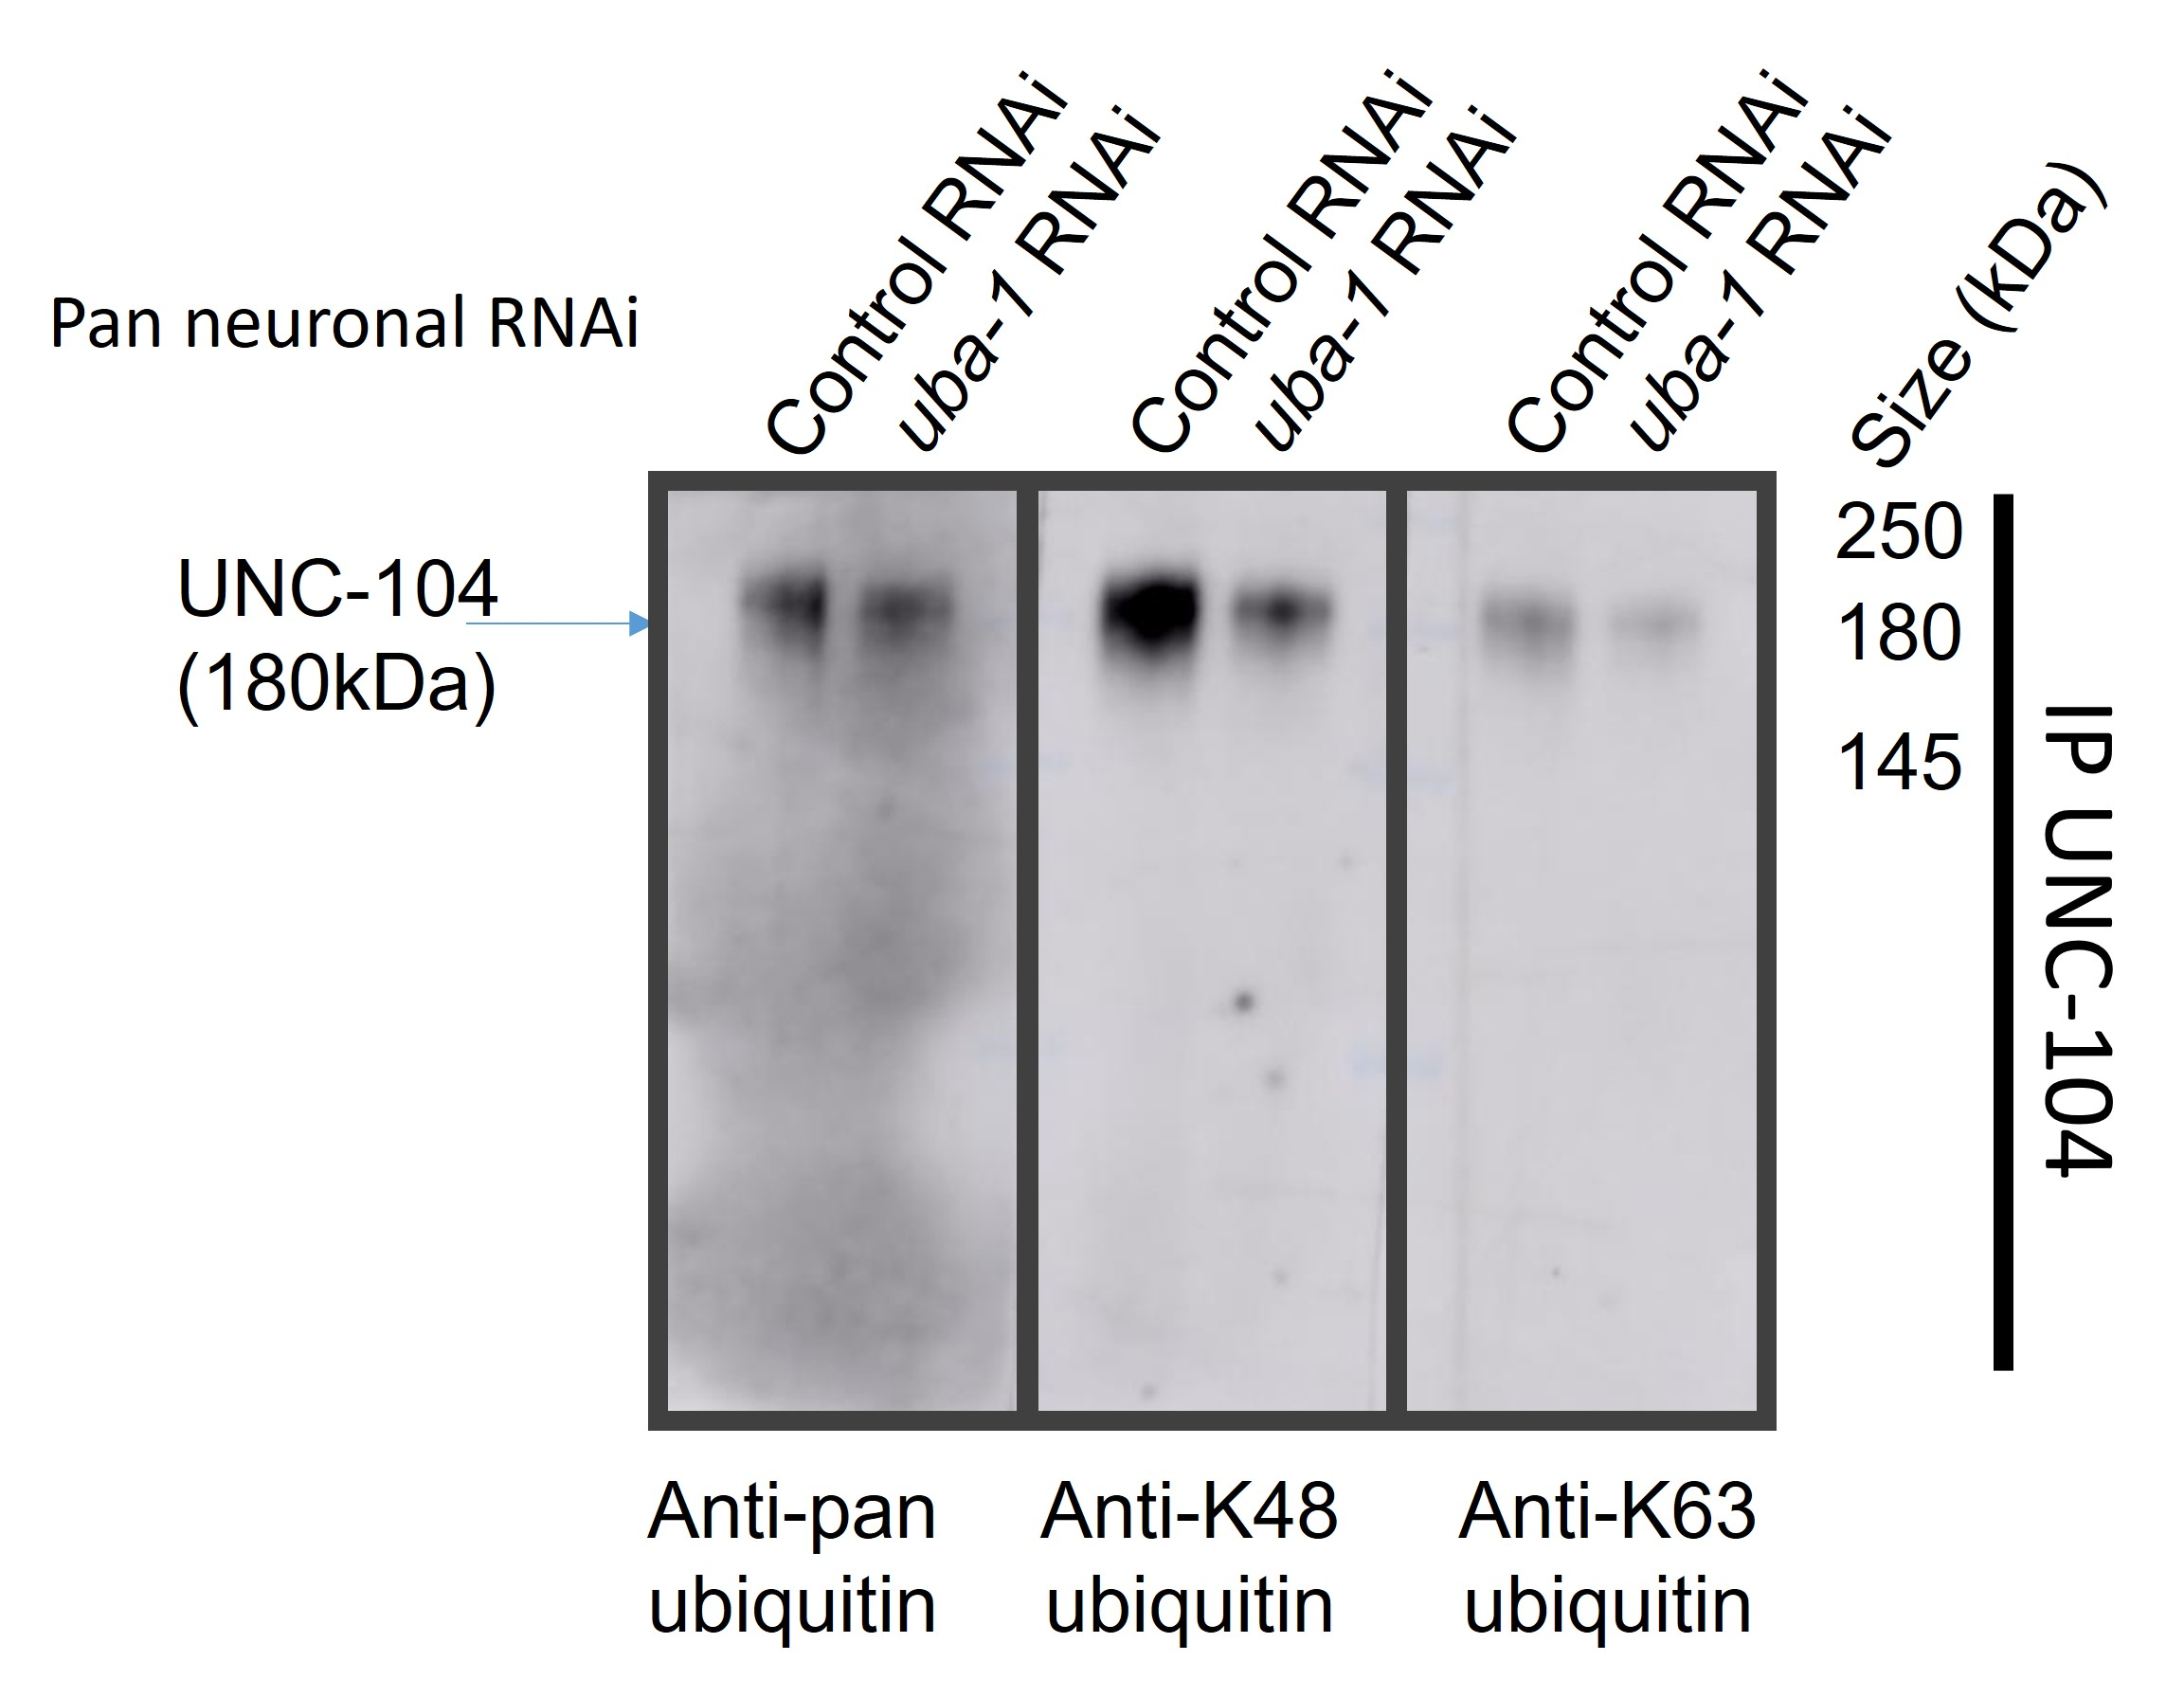
\includegraphics[width=\textwidth]{figs/example}
	
	\caption[Mechanism that contribute to compartment specific transport.]{\textbf{Mechanism that contribute to compartment specific transport.}} \raggedright \small Schematic representation of different examples of mechanisms that may regulate location specific transport of various kinesin members in a neuron. The mechanisms include 1) differentially modified MT indicated as red and blue lines that drive selective transport, 2) the axon initial segment (AIS) marked in the proximal axon that may act as a selective barrier, and 3) enrichment of kinesins at particular locations such as within the cilia.
 	\label{fig:Ch1f1}
\end{figure}

You can use an acronym by the gls command \gls{NRX-1}. Only after referencing an acronym will it show in the acronym list.

You can also use math symbols such as $\sim$10 $\mu$m.

You can reference a figure using [Fig.~\ref{fig:Ch1f1}]. A similar code can be used for an element you label using the label command.

You can also leave a personal comment using \marginpar{Neuronal migration?}.

You can leave bullet points with:-
\begin{enumerate}
	\item First point 
	
	\item Second point

	\item Third point

\end{enumerate}


Equations can be added in Latex format
\begin{equation}
	\label{dyn2}
	\partial_t \frac{C(x,t)}{C_{0}} + v \partial_x \frac{C(x,t)}{C_{0}}  - D \partial_x^2 \frac{C(x,t)}{C_{0}}  = 0, \nonumber
\end{equation}

These equations can be referenced [Fig.~\ref{dyn2}]. 

\textcolor{red}{You can highlight text using this command}

You can also add equations inline using  $\frac{C(x,t)}{C_{0}}$. i

\section{Table Example}
\blindtext \index{example2}

You can add a table using the following format.
\begin{table}[ht]
	\centering
	\caption{Closest orthologue of selected E3s} \label{tab:E3sselected}
	\begin{tabular}{|c|c|c|}
		\hline 
		Phenotype	& \textit{C. elegans} gene& Closest mammalian orthologue \\[0.5ex] 
		\hline\hline 
		Distal end UNC-104 accumulation	& \textit{fbxa-81} & FBXL13 \\ 
		\hline 
		Distal end UNC-104 accumulation	& \textit{fbxb-65} & FBW1A\\ 
		\hline 
		Distal end UNC-104 accumulation	& C10E2.2& FBXO30\\ 
		\hline 
		Synapse UNC-104 accumulation & \textit{fbxb-35}& NIL\\ 
		\hline 
		Synapse UNC-104 accumulation & \textit{fbxa-103}& NIL\\ 
		\hline 
	\end{tabular}
	
\end{table}
\blindtext 


A specially formatted table that have different column widths and can continue for multiple pages
\newcolumntype{L}{>{\RaggedRight\hangafter=1\hangindent=1.5em}X}
\begin{table}[H]\centering
	\caption{Strain list used in this chapter}\label{tab:Strainlist2}
	\scriptsize
	\begin{tabularx}{1\textwidth}{@{} l l L l @{}}\toprule
		S. No. &Strain name &Genotype &Reference \\\midrule
		1 &NM2689 &\textit{jsIs821 [mec-7p::gfp::rab-3]} &\cite{bounoutas2009} \\
		2 &NM3764 &\textit{jsIs1111 (mec-4p::unc-104::gfp)} &\cite{kumar2010} \\
		3 &TU3568 &\textit{sid-1(pk3321) him-5(e1490)} V; \textit{lin-15B(n744)} X; \textit{uIs71 [(pCFJ90) myo-2p::mCherry + mec-18p::sid-1]} &\cite{calixto2010} \\
		4 &RV110 &\textit{uba-1(it129ts)} &\cite{kulkarni2008} \\
		5 &TT343 &\textit{tbIs147} [Integrated line of \textit{mec-4p::UNC-104::GFP} in e1265 background] &\cite{kumar2010} \\
		6 &TT2980 &\textit{tbEx409 [mec-4p::mScarlet]} &This study \\
		7 &TT2228 &\textit{tbEx275} [\textit{mec-4p::UNC-104::GFP}(TTpl506)(5ng/ul) + \textit{ttx-3p::RFP}(TTpl541)(50ng/ul)+ pBluescript SK-(TTpl542)(200ng/ul)] &This study \\
		8 &TT2319 &\textit{tbEx276} [\textit{mec-4p::UNC-104 deltaPH::GFP}(TTpl567)(5ng/ul) + \textit{ttx-3p::RFP}(TTpl541)(50ng/ul)+ pBluescript SK-(TTpl542)(200ng/ul)] &This study \\
		9 &TT2353 &\textit{tbEx281} [\textit{mec-4p::UNC-104(M1540I)::GFP}(TTpl570)(5ng/ul) + \textit{ttx-3p::RFP}(TTpl541)(50ng/ul)+ pBluescript SK-(TTpl542)(200ng/ul)] &This study \\
		10 &TT2355 &\textit{tbEx279} [\textit{mec-4p::UNC-104(D1497N)::GFP}(TTpl569)(25ng/ul) + \textit{ttx-3p::RFP}(TTpl541)(50ng/ul)+ pBluescript SK-(TTpl542)(100ng/ul)] &This study \\
		11 &TT2399 &\textit{tbEx287} [\textit{mec-4p::UNC-104(D1497N M1540I)::GFP}(TTpl578)(3ng/ul) + \textit{ttx-3p::RFP}(TTpl541)(50ng/ul)+ pBluescript SK-(TTpl542)(200ng/ul)] &This study \\
		12 &TT2398 &\textit{tbEx289} [\textit{mec-4p::GFP}(TTpl581)(1ng/ul) + \textit{ttx-3p::RFP}(TTpl541)(50ng/ul)+ pBluescript SK-(TTpl542)(200ng/ul)] &This study \\
		13 &TU3401 &\textit{sid-1(pk3321) uIs69 [(pCFJ90) myo-2p::mCherry + unc-119p::sid-1]} V &\cite{calixto2010} \\
		\bottomrule
	\end{tabularx}
\end{table}


% After each chapter you can add biblography.
% If you want only one Biblography, remove following helper file and put content of it in main.tex
%\clearpage
%% This is helper file which you can use in every chapter if you want to have separate biblography for each chapter

% If you want only single biblography for all thesis, just copy paste following content at the end of main.tex

%	\bibliographystyle{unsrt}
%	\bibliography{Thesis}

	\printbibliography
	
% Material and methods
%\begin{appendices}
	
\chapter{Material and Methods}

\section{Maintenance of \textit{C. elegans} on agar and in liquid}

Worms were maintained on NGM agar at 20\textsuperscript{o}C \parencite{brenner1974}. All images unless specified otherwise were taken from worms at the L4 stage. We use cell-specific SID-1 (a ds-RNA transporter) overexpression along with a sid-1 mutant as previously standardized for both TRN-specific and pan-neuronal RNAi to ensure most efficient RNAi in neurons \parencite{calixto2010}. For all imaging experiments treated with RNAi, we used a strain with the required markers built with the TRN-specific RNAi sensitive strain expressing SID-1 expressed under the ¬mec-18 promoter, which only expresses within the 6 TRNs. For all biochemistry experiments treated with RNAi, we used a strain with the required marker built with the pan-neuronal RNAi sensitive strain expressing SID-1 under the pan-neuronal unc-119 promoter. For biochemistry experiments, worms were maintained for a maximum of 1 generation in liquid culture to increase the biomass available. A liquid culture was started by harvesting worms from 5 almost starved plates based on a modified protocol from \parencite{shaham2006}. In brief, the liquid culture is composed of S basal [5.85 g NaCl, 1 g \ce{K2HPO4}, 6 g \ce{KH2PO4}, 1 ml cholesterol (5 mg/ml in ethanol), \ce{H2O} to 1 liter. Sterilize by autoclaving.]. 1L S medium was made from S basal by addition of the following components prior to use, 1 M Potassium citrate pH 6.0 [20 g citric acid monohydrate, 293.5 g tri-potassium citrate monohydrate, H2O to 1 liter. Sterilize by autoclaving.] and Trace metals solution [1.86 g disodium EDTA, 0.69 g \ce{FeSO4.7 H2O}, 0.2 g \ce{MnCl2.4 H2O}, 0.29 g \ce{ZnSO4 .7 H2O}, 0.025 g \ce{CuSO4 .5 H2O}, \ce{H2O} to 1 liter. Sterilize by autoclaving. Store in the dark.], and 1 M \ce{CaCl2} [55.5 g \ce{CaCl2} in 1 liter \ce{H2O}. Sterilize by autoclaving.]. The composition of S medium was [1 liter S Basal, 10 ml 1 M potassium citrate pH 6, 10 ml trace metals solution, 3 ml 1 M \ce{CaCl2}, 3 ml 1 M \ce{MgSO4}; do not autoclave.]. The S medium was used as a buffer to wash the worms off the plate and grown in glass round bottom test tubes at 20\textsuperscript{o}C with 180 rpm shaking. After adding the worms to the S medium, concentrated \textit{E. coli} OP50 pellet to a final concentration of 30g/L, washed and diluted in S medium was added. If a synchronized culture is needed, the almost starved seed plates were additionally treated with a 4\% bleach solution (1:1 ratio of 1N NaOH:4\% Sodium hypochlorite). The eggs were then used as seed for the liquid culture.

\section{RNAi screen in \textit{C. elegans}}

An overview of E3 ligases in \textit{C. elegans} suggests that there are $>$550 distinct E3 ligases present among various classes \parencite{jin2004, kipreos2000, passmore2004}. Due to the infeasibility of screening so many E3s, we decided to narrow the scope of the screen based on neuronal expression of the E3s. This subselection was based on a 2 part selection. The list of E3s was gathered from Wormbase \parencite{howe2016} via a custom developed Python script [Code~\ref{lst:E3list}] scraping gene coding sequences containing known E3 ligase domains, such as the F-box and RING-containing ligases. The CDS of sequences associated with these E3s were then gathered from NCBI. Each of these sequence files were then aligned with previously published single cell RNA-seq databases \parencite{hutter2016}, which attributed RNA expression levels in different tissues as well as in different types of neurons. This list of relative expression was used to select only E3s that are expressed in neurons, followed by an expression in at least the 6 mechanosensory TRNs as estimated by the sequence read archive (NCBI) runs ["SRR2969242", "SRR2969241", "SRR2969240", "SRR2969239", "SRR2969238", "SRR2969237", "SRR2969236"]. A large fraction of these E3s comprise the F-box family of proteins, which act together with the SCF complex to target proteins to ubiquitination \parencite{kipreos2000}.

We utilized the Ahringer library \parencite{kamath2003} of \textit{E. coli} HT115 expressing dsRNA against $\sim$90\% of the \textit{C. elegans} protein coding genes. The final list of \textit{E. coli} expressing dsRNA against 95 E3s that were present in the Ahringer library were rescued by growing in LB with 20 mg/ml tetracycline and 100 μg/ml ampicillin. The selected E3s were sent for sequencing to confirm the presence of the specific E3 targeting sequence.

To induce dsRNA expression, two methods were used. For growing \textit{C. elegans} on agar, a primary culture of the dsRNA containing \textit{E. coli} was grown in LB with 100 μg/ml ampicillin for 12 hours at 37\textsuperscript{o}C. After 12 hours, 500 μL of this broth was spotted on NGM agar supplemented with 1 mM IPTG and 10 mg/ml ampicillin. The plate was rapidly dried by leaving the lid open in a laminar air flow. After drying of the bacterial spot, the plates were incubated for at least 1 day at 20\textsuperscript{o}C before placing \textit{C. elegans} on them. The worms were then imaged after 4 days when the F1 progeny reached the L4 stage. The spotted plates were used for a maximum of 4 days after being spotted due to increased variability observed in the phenotypes after that time.

We utilised the previously published neuronal RNAi sensitive strain, which expresses the dsRNA transporter, SID-1, specifically in the TRNs. Previous studies have suggested that overexpression of SID-1, along with mutated somatic lin-15 and sid-1, leads to $>$90\% knockdown of gene expression in the TRNs \parencite{calixto2010}. One caveat of using RNAi by feeding HT115 expressing dsRNA is that it takes $\sim$18 hours for RNAi to initiate. In terms of development, this is enough time for \textit{C. elegans} to reach early L3 post hatching. Thus to maintain consistency, we grew \textit{C. elegans} from embryos to mid L4 on dsRNA expressing bacteria before observing and annotating UNC-104 accumulation. Thus, we used the strain \textit{sid-1(pk3321)}, \textit{him-5(e1490)}; \textit{uIs71(mec-4p::SID-1)}; \textit{jsIs1111(mec-4p::UNC-104::GFP)}; \textit{lin-15B(n744)} to enhance the RNAi induced knockdown of genes. 

To build the strain and confirm \textit{sid-1(pk3321)} homozygous mutants after selecting for plates throwing high incidence of males (\textit{him-5(e1490)} homozygous phenotype), we used resistance against knockdown of the embryonic lethal gene \textit{dyci-1}. 10 individual animals were separated on \textit{dyci-1} RNAi 24 well plate and no lethality observed in any well was inferred to be homozygous for \textit{sid-1(pk3321)}. Selection of \textit{lin-15B(n744)} depended on the homozygous temperature sensitive phenotype. A 24 well plate with putative \textit{lin-15B(n744)} homozygous animals were replicated on another 24 well plate, and this plate with the adults was places at 25\textsuperscript{o}C. It is important to note that temperature sensitivity was only observed before the worms reached the L2 stage. Complete lethality was inferred as the well being homozygous for \textit{lin-15B(n744)}.

For biochemistry experiments relying on RNAi, the primary culture of the dsRNA containing \textit{E. coli} were grown for 14 hours at 37\textsuperscript{o}C in LB with 10 mg/ml ampicillin. A secondary culture was initiated after 14 hours using a 1\% inoculum of the primary culture in pre-warmed LB containing 1mM IPTG and 10 mg/ml ampicillin. This culture was grown for $\sim$5 hours at 37\textsuperscript{o}C till 0.6 O.D. at which point, the bacteria was pelleted at 3000 $\times$g for 10 min and washed twice with the S medium. Finally, the bacterial pellet was resuspended in S medium supplemented with 1mM IPTG and 10 mg/ml ampicillin and added to the liquid culture at a concentration of 30 mg/ml. Occasionally for very large worm cultures, an additional supplement of bacteria was given after 2 days if the liquid culture started appearing very clear to avoid worms undergoing starvation.

\textit{C. elegans} neurons are generally resistant to RNAi. Thus, to enhance the knockdown of our genes of interest, we used a previously published mutant of \textit{sid-1} along with overexpressing SID-1 in the neurons of our interest. For TRN specific imaging, we used the strain \textit{sid-1(pk3321) him-5};\textit{uIs71};\textit{lin-15B} built with the transgene of our interest [Table~\ref{tab:Strainlist2}]. For biochemistry experiments, we used the pan neuronal strain \textit{sid-1(qt2)};\textit{uIs69} built with our markers of interest.

Worms were screened under a Nikon Ti-70 upright epifluorescence microscope in 20$\times$/ 0.8 N.A. air objective, with worms anesthetized in 5 mM tetramisole and laid on a 5\% agarose pad. Intensity of UNC-104::GFP was manually entered within a range of 1-5 in the PLM and ALM at the cell body, neuronal process 100 $\mu$m away from the cell body, the branch, the synapse and the distal ends. This scale was calibrated based on the least fluorescence excitation required for UNC-104::GFP intensity to be visible by eye based on presence of ND filters within the light-path. ND0 (100\% transmission) corresponds to 1, ND2 ($\sim$50\% transmission) corresponds to 2, ND4 ($\sim$25\% transmission) corresponds to 3, ND8 ($\sim$12.5\% transmission)  corresponds to a grade of 4, and ND16 ($\sim$6.25\% transmission) correspond to a grade of 5.

The intensity of 95 E3s, 12 E2s and 1 E1 were plotted on a heat map along with a GFP RNAi and an Empty Vector L4440 RNAi control. The heat map was clustered based on the intensity at different regions using Python’s Seaborn module cluster-map \parencite{waskom2021}. Broadly, most of the RNAi targeting E3s clustered along with the Empty Vector and were not used further. The RNAi that showed a phenotype fell in 1 of 3 categories, 1) with UNC-104::GFP high everywhere, 2) with UNC-104::GFP high in the distal end and low in cell body, and 3) with UNC-104::GFP high at synapses and the cell body.

\section{Imaging of \textit{C. elegans}}

Worms at the L4 stage were imaged using 5 mM tetramisole anesthetic and mounted on a 5\% agarose pad solidified on a microscope slide unless otherwise stated.

\subsection{LSM710 ablation imaging}
Imaging immediately post ablation was done on a Zeiss LSM 710 with a 63$\times$/1.4 DIC oil objective at 3$\times$ zoom leading to a pixel size of 90 nm with illumination from a 488 nm Argon laser. Images were acquired every 500 ms in the ALM and PLM around 70 μm or 280 μm away from the cell body. Ablation was done in the Zen software using a femtosecond MaiTai Ti: Sapphire laser (Spectra-Physics) mode locked at 800 nm at 80\% power (400 mW at objective calculated at 10$\times$) with 20 iterations post acquiring 5 pre-bleach images. The imaging was done for at least 200 frames post-bleach.

Post-acquisition, movies were analyzed using FIJI, by drawing a rectangular ROI of around 1$\times$2 μm to cover the proximal and distal cut-site. The intensity at each time point was exported along with the ROI of bleaching and the ablation time point. The data was then normalized to pre-ablation intensity values and plotted with an in-house script generated in Python.

\subsection{LSM880 FRAP and protein distribution imaging}

Imaging to calculate the diffusion kinetics and calculating the distribution of UNC-104::GFP in the neuron was carried out in a Zeiss LSM 880 equipped with a 40$\times$/1.4 N.A. DIC oil objective at 2$\times$ zoom leading to a pixel size of 208 nm. Due to the need of fast imaging and high sensitivity, a GaAsP high sensitivity detector was used to capture signal from a worm illuminated with a solid state 488 nm Argon LASER at 5\% power (4 mW max at objective) scanned with a resonant scanner. Since the neuron was majorly present as a straight line, the frame size was reduced in the y-axis to 50 pixels and the x-axis to 512 pixels that encompassed only the neuron of interest. The frames were averaged 2$\times$ based on fly back line averaging to improve signal sensitivity. Photobleaching was optimized by using 80\% 488 nm illumination in a region of around 50 μm in the neuronal process iterated 5 times over the region. 5 frames were taken pre-photobleaching and the animal was imaged for at least another 180 seconds post-photobleaching.

Post-acquisition, movies were analyzed using FIJI, by importing the rectangular ROI used for photobleaching. The intensity of UNC-104::GFP was calculated by drawing a line tracing the neuron and exporting the distance and intensity of each time point along with the boundaries of bleaching and the bleaching time point. The data was then normalized to pre-photobleaching intensity values and plotted with an in-house script generated in Python.

To image UNC-104::GFP distribution, we used LSM 880 equipped with a 63$\times$/1.4 N.A. oil objective at 1024$\times$1024 pixels leading to a pixel size of 88 nm using a high sensitivity GaAsP detector illuminated with 488 nm argon LASER and imaged with a spectral filter from 493 to 555 nm. The entire length of the neuron was then imaged by tiling across 6 regions with a 10\% overlap at 5\% LASER power at 488 nm and 2$\times$ flyback linescan averaging. Simultaneously, mScarlet was imaged using a spectral filter from 585 to 688 nm with a 561 nm DPSS LASER at 5\% power at the same resolution.

The images were automatically stitched using the Zen software. A line profile starting from the distal end of the PLM was traced till the cell body and the intensity and distance data were exported and analyzed using an in-house script generated in Python.

\subsection{Hamamatsu spinning disc with Volocity}

UNC-104::GFP and GFP::RAB-3 particle tracking were imaged on an Olympus IX83 microscope equipped with a spinning disc Yokogawa CSU-X1 module leading to a Hamamatsu EM-CCD camera. The worms were illuminated by a 488 nm solid state LASER at 15\% LASER power (1 mW maximum output at 100$\times$) and imaged using a 100$\times$/1.4 N.A. oil objective with an effective pixel size of 0.129 μm/pixel. The exposure time was set to 300 ms which gave an effective frame rate of 3 frames per second. The movies were taken for a minimum of 3 mins and a maximum of 5 mins and imaged in the PLM around 70 μm or 280 μm away from the cell body. 

\subsection{GCaMP imaging}

The strain \textit{ljSi2}[\textit{mec-7p::GCaMP6m::SL2::tagRFP}]; \textit{zfIs42}[\textit{rig-3p::GCaMP3::SL2::mCherry}] was imaged using the conditions stated above near the PLM synapses. A $1 \times 1  \mu m^2$ region around 1 $\mu$m juxtaposed but not overlapping to a portion of the PLM branch $\sim$20 $\mu$m from the PLM synapse was exposed with 100\% LASER power (1 mW maximum output at 100$\times$) for 10 iterations. Intensity quantification for the PLM synapses was done using an manual ROI $\sim 3 \times 2$ $\mu m^2$ drawn over the PLM synapses that did not visibly overlap with the AVA process. Similarly, intensity for the AVA process was calculated using a $5 \times 1  \mu m^2$ ROI drawn along the AVA process juxtaposed to the PLM synapse but not overlapping [See schematic of Fig.~\ref{fig:GCaMPubs}]. The photo-activation time-points were extracted from the image metadata using a custom ImageJ macro. The AVA demonstrated 2 distinct intensity levels consistent with what is expected of a plateau potential. The AVA did not respond to activation of the PLM while the AVA was at the lower intensity GCaMP phase [Fig.~\ref{fig:GCaMPintro}]. Thus, to average intensity across multiple trials, a secondary threshold for the AVA intensity $\sim$40\% of the maximum observed intensity was used to separate the data and only the trials with the higher AVA intensity was used in the plots shown. The mean $\pm$ S.D. was plotted with the stimulation time aligned with 10 pre-stimulation frames and 45 post-stimulation frames plotted. 

\subsection{Prime-EM spinning disc with cellsens}

UNC-104::GFP and GFP::RAB-3 particle tracking in the CRISPR generated mutants \textit{unc-104(syb7293)} and \textit{fbxb-65(syb7320)} were imaged on an Olympus IX83 microscope equipped with a spinning disc Yokogawa CSU-W1 module leading to a Prime BSI back illuminated sCMOS camera. The worms were illuminated by a 473 nm solid state LASER at 15\% LASER power (1 mW maximum output at 100$\times$) and imaged using a 100$\times$/1.4 N.A. oil objective at 2$\times$ binning with an effective pixel size of 0.13 μm/pixel. The exposure time was set to 300 ms which gave an effective frame rate of 3 frames per second. The movies were taken for a minimum of 3 mins and a maximum of 5 mins and imaged in the PLM around 70 μm away from the cell body. 

\subsection{Kymograph analysis}

The movies were analyzed by tracing the neuron using the segmented line tool in FIJI and generating kymographs using the kymograph plugin \parencite{katrukha2020}. The kymograph was then traced manually for visually distinct tracks and analyzed using an in-house FIJI macro. The estimated vesicle properties were then analyzed by custom visualizations in Python.

Analysis of UNC-104::GFP tracks intensity was carried out by measuring the average intensity of the previously traced kymographs. The intensity of the lines was then background subtracted by shifting the traced lines 4 pixels up ($\sim$1.3 seconds before the particle passed) and subtracting this averaged value from the particle intensity. The average background subtracted intensity was then plotted and analyzed.

\subsection{Fluorescence correlation spectroscopy}
Fluorescence correlation spectroscopy was performed on an IX83 scope with a 60$\times$/1.1 N.A. water objective illuminated with a 488 nm solid state LASER and equipped with a photon counting detector from PicoQuant PMA Hybrid Photomultiplier detector. The correction collar was adjusted to gain the maximum intensity from GFP fluorescence in the neuronal process. The ROI was parked in the middle of the neuronal process around 70 μm away from the cell body. The autocorrelation function was then calculated using data aggregated from the ROI for 1 min using the PicoQuant SymPhoTime 64 software.

The autocorrelation function $G(t)$ was analyzed using custom Python scripts in two ways to yield information about the number and nature of the diffusing species. The first method relied on the maximum entropy data fitting of the autocorrelation function using the equation \parencite{sengupta2003}
\begin{equation}
	\label{eqn:autocorrelation}
	G(t) = \sum_{a=0}^{n}\frac{a_{n}}{n}\sqrt{\frac{1}{1+\frac{t}{\tau}}}
\end{equation}

Where $n$ is the total number of residence times tested, a is the contribution of that residence time to the fitting, $\tau$ is the estimated residence time. The data was fit using Python’s Least-Squares Minimization routine lmfit package \parencite{newville2014}. Using this method, 2 distinct diffusing species were best fit for data from UNC-104::GFP while only 1 diffusing species was best fit for soluble GFP. The average residence time $\tau$ was then used to get an estimate of the fraction of diffusing species in that residence time using the equation
\begin{equation}
	\label{eqn:autocorrelationall}
	G(t) = a_1\sqrt{\frac{1}{1+\frac{t}{\tau_1}}} + a_2\sqrt{\frac{1}{1+\frac{t}{\tau_2}}}
\end{equation}

Where $a_1$ and $a_2$ are the relative contributions of the diffusing species to the autocorrelation function $G(t)$, and $\tau_1$ and $\tau_2$ are their respective correlation times.

\subsection{IX73 and ablation}

Worm ablation and imaging 1 hr post ablation were carried out on a modified dual-deck IX73 epifluorescence microscope. The upper deck was attached to a Q-switched Nd:YAG LASER (Minilite II, 4-ns pulse- width, $\lambda$ = 355 nm, Continuum). 3-5 seconds of exposure of the LASER with the neuron in focus was used to ablate the neuron with minimal injury to the surrounding tissues. Ablation was confirmed by loss in fluorescence in the ablated area which does not recover up to 1 min post-ablation. The animals were then rescued on NGM OP50 plates and noted for the side that was ablated. 1 hr later, the same side of the worm was loaded on a slide and imaged. The worms were illuminated with 100\% output from a 120W X-cite mercury-arc lamp and imaged using a Photometrics Evolve 512 EMCCD camera.

The intensity of the 1 μm region juxtaposed to proximal and distal cut-site was calculated using FIJI and normalized to the intensity 10 μm away. The intensity was then plotted using custom visualization scripts written in Python

\section{Biochemistry of \textit{C. elegans}}

Worm biochemistry was conducted by growing worms in liquid culture for 1 generation as previously described. After achieving the correct stage, worms were harvested by spinning in conical tubes at 300 $\times$g for 30 seconds, followed by 3 successive washes in the M9 buffer. The worms were then resuspended in twice the worm bed volume of Homogenization Buffer [15 mM HEPES pH 7.6, 10 mM KCl, 1.5 mM \ce{MgCl2}, 0.1 mM EDTA, 0.5 mM EGTA, 44 mM Sucrose and 100 mM NaCl] supplemented with 1x EDTA free Complete Protease Inhibitor Cocktail (Sigma). For experiments that required probing ubiquitin, 20 mM NEM was also added to the Homogenization buffer to prevent deubiquitinase activity. This worm solution was flash frozen and stored until further use unless otherwise stated. If protein lysates needed for IP or SV preps, the frozen worm pellets were thawed on ice and disrupted using a bath sonicator (bioruptor). We used 5 iterations of 30 s on and 20 s off pulses at 100\% power. This lysate was then spun at 1000 $\times$g for 10 mins at 4\textsuperscript{o}C to get rid of the worm carcasses and insoluble matter. The supernatant was separated and used as required.

\subsection{Western blotting}

Protein lysate was boiled in Laemmli buffer at 95\textsuperscript{o}C for 5 mins just prior to loading on a gel. The gel was cast at 8\% resolving for the full UNC-104 protein, and 12\% resolving for the fragments of UNC-104 individually expressed, with a 5\% stacking gel overlayed. The gels were run in 1x Running buffer, at 90 V while in stacking, and at 120V in resolving. After sufficient resolving, the proteins were wet transferred onto a supported nitrocellulose membrane at 250 mA for 100 mins, followed by probing with Ponceau S stain. After probing for correct transfer, the blots were blocked with 5\% skimmed milk dissolved in PBS+0.1\% Tween 20 for 1 hr at room temperature. After blocking, the primary antibody was diluted in 5\% BSA with PBST (0.1\% Tween 20 in 1x PBS) and added as per \textcolor{black}{1) mouse anti-UNC-104 antibody (25H11E6) (1:40) (Self generated and maintained by Bioklone, Chennai, India) incubated at 4\textsuperscript{o}C for $>$8 hrs, 2) mouse anti-ubiquitin antibody (FK2) (1:1000) (acquired from Sigma-Aldrich, India) incubated  at 4\textsuperscript{o}C for $>$8 hrs, 3) mouse anti-myc (AE010) (1:5000) (manufactured by ABclonal, acquired from Allianz BioInnovation, Mumbai, India) incubated at room temperature for 1.5 hours, 4) mouse anti-actin (AC004) (1:5000) (manufactured by ABclonal, acquired from Allianz BioInnovation, Mumbai, India) incubated at room temperature for 1.5 hours, 5) HRP Goat Anti-Mouse (AS003) (1:5000) (manufactured by ABclonal, acquired from Allianz BioInnovation, Mumbai, India) incubated at room temperature for 1.5 hours.}

After antibody incubation, the blots were washed thrice with PBST for 10 mins with rapid rocking. After secondary antibody incubation, the blots were developed with SuperSignal™ West Femto Maximum Sensitivity Substrate and imaged in a GE chemidoc system. For quantification, UNC-104 band intensity was measure by drawing a rectangle over the band and measuring the same are just above the band of interest that serves as the background. These background subtracted intensities were normalized to the control actin background subtracted intensities derived from the same blot.

\subsection{Immunoprecipitation}

Immunoprecipitations (IP) were conducted in the IP buffer, which is Homogenization buffer as described before + 100mM NaCl. Briefly, ChromoTek Myc-Trap® Agarose \textcolor{black}{(acquired from Everon Life Sciences, New Delhi)} were resuspended and washed thrice in PBS followed by equilibration thrice in IP buffer for 10 mins each at 4\textsuperscript{o}C. After equilibration of beads, the beads were distributed into tubes containing 5mg whole worm lysate. These tubes were then left at a rotation speed of 30 rpm at 40 \textsuperscript{0}C for 4 hours. After 4 hours, the beads were gently pelleted using gravity and washed thrice with IP buffer for 10 mins. Finally, the beads were resuspended in 20 μL IP buffer + Laemelli buffer and boiled at 95\textsuperscript{o}C for 5 mins.

\subsection{Antibody - Protein G agarose beads crosslinking}

For experiments that relied on the same antibody for probing and IP, the antibody was cross-linked to Protein G bound agarose beads to prevent detection of the antibody heavy chain on a western. Protocol for antibody cross-linking with protein-G coupled beads was adapted from \cite{harlow1988}. Briefly, the protein-G coupled beads were equilibrated with PBS and added to antibody ascites, or desired amount of antibody was added to the protein-G beads in PBS solution. Antibody bound protein-G agarose beads were then equilibrated in a conjugation buffer [0.2 M Sodium borate buffered at pH 9.0 in \ce{H2O}] by washing thrice in 10$\times$ the volume. The final harvested beads were resuspended in 20 mM dimethylpimelidate (DMP) made fresh in the same conjugation buffer. This solution was slowly rotated for 30 mins at room temperature to prevent the beads from settling. The crosslinking reaction was stopped by adding 10$\times$ volume of 0.2M ethanolamine (pH 8.0), followed by 1 wash with 0.2M ethanolamine (pH 8.0) and incubation for 2 hours at room temperature with slow revolving. The beads were then washed with 10$\times$ volume of PBS thrice to remove all traced of ethanolamine. The final PBS diluted protein-G coupled antibodies can then be used directly after proper equilibration, or stored with 0.02\% sodium azide in PBS for up to 1 month. 

\subsection{Synaptic Vesicle preparations}

SV preps were made from the lysates of the homogenized worms described above. A few modifications included, a reduction of the iterations of sonication from 5 to 3, and manual homogenization using a micropestle (10 rounds). After disruption, the worm pellets were spun at 1,000 $\times$g for 10 mins at 4\textsuperscript{o}C to get rid of the worm carcasses followed by another spin at 10,000 $\times$g for 20 mins at 4\textsuperscript{o}C to get rid of heavy membrane fractions such as nuclear and mitochondrial fractions. A final spin at 100,000 $\times$g at 4\textsuperscript{o}C for 2 hours separated synaptic vesicle protein containing fractions from a soluble protein fraction. These supernatant and pellet fractions were used to quantify synaptic vesicle bound and unbound protein levels. Quantification of intensities were carried out as described above. For normalization, the background subtracted pellet intensities were divided by the background subtracted input intensities of UNC-104 and actin separately. The normalized UNC-104 intensity was further divided by the normalized actin intensity to get a value compared across trials.

\subsection{Sucrose density gradient separation}

In case SVs need to be purified away from other vesicular fractions, we used a sucrose density gradient. Different sucrose concentrations were made in MEPS buffer (35 mM PIPES, 5 mM EGTA, 5 mM \ce{MgSO4}, pH 7.1) at concentrations of 0 M, 0.2 M, 0.5 M, 1 M, and 1.5 M. These concentrations were layered gently using a cut 1 ml tip in an open-top thin walled polypropylene tube, with 0.75 ml of each dilution in a layer with the highest concentration at the bottom. The worm lysates were prepared in MEPS buffer, homogenized, and spun at 1,000 $\times$g for 10 mins at 4\textsuperscript{o}C. These lysates were directly layered on top of the prepared sucrose gradient along with pre-equilibrated Cospheric density marker beads (DMB-kit-7 (1.02, 1.04, 1.06, 1.08, 1.09, 1.13, 1.38g/cc)). This gradient was spun in a pre-chilled swing bucket MLS-50 Beckman Coulter ultracentrifuge at 100,000 $\times$g for 2 hours at 4\textsuperscript{o}C. After the run, different interfaces were visualized using the density gradient beads and separated using aspirating in a 22 gauge syringe needle. The resulting solutions were diluted 10$\times$ with 0 M sucrose MEPS buffer and centrifuged again at 100,000 $\times$g for 1 hour at 4\textsuperscript{o}C. The supernatants were discarded and the pellets were resuspended in 0 M sucrose containing MEPS buffer and boiled with Laemelli's buffer before loading it on a western. Synaptic vesicles are generally observed in the interface between 0 and 0.2 M sucrose, while soluble proteins are observed after 1 M sucrose.

\section{Statistics}

Statistical analyses were performed using GraphPad Prism 9 or the SciPy stats module v1.11.2 of Python 3.8 \parencite{virtanen2020}. The Shapiro–Wilk test was used to examine the normality of various distributions. Sample size estimates were calculated using G*Power 3.1.9.7 \parencite{faul2007} or via previously published literature. Single comparisons between normally distributed data were performed using unpaired two-tailed Student’s t-test and those between non-normal distributions were performed using the Mann–Whitney U test. For multiple comparisons, one-way ANOVA with Dunnett’s multiple comparisons test was used for normal data, and Mann–Whitney–Wilcoxon test with Bonferroni multiple comparisons correction was used for non-normal data. Data were represented either as Median with the 25\textsuperscript{th} and 75\textsuperscript{th} percentiles labeled, or as Mean $\pm$ S.D.


\section{Molecular Biology}

\subsection{qPCR}

RNA was isolated from worms by the Trizol method. A worm pellet was harvested by 3 serial washes of an almost starved plate with M9 followed by resuspension of the worms in 10$\times$ volume of Trizol. This solution was frozen at -80\textsuperscript{o}C until further use. When needed, the trizol was rapidly thawed and vortexed for 5 mins. To 1 ml of this solution, 200 μL of fresh chloroform was added and vortexed for 30 s. The solution was then allowed to phase separate at room temperature and spun at 10,000 $\times$g for 10 mins at 4\textsuperscript{o}C. The aqueous phase was separated and a 1:1 ratio of isopropanol was added. This solution was gently flipped to mix and left at -20\textsuperscript{o}C for 4 hours. After 4 hours, the solution was spun at 10,000 $\times$g for 10 mins at 4\textsuperscript{o}C. The supernatant was thrown and the pellet was washed by flipping with 70\% ethanol till the pellet broke apart. The solution was spun at 10,000 $\times$g for 10 mins again. The resulting supernatant was discarded and the pellet was air dried. The pellet was finally dissolved in nuclease free water and quantified using a NanoDrop™ One/OneC Microvolume UV-Vis Spectrophotometer. Simultaneously the RNA quality was checked on an 1\% agarose gel. If 2 distinct bands are observed with minimal degradation of RNA, 1 μg of this RNA was taken and converted to cDNA using Superscript IV RT polymerase via the manufacturers protocol with random hexamers. The resultant cDNA was diluted 1:20 and used for qPCR reactions.

For qPCR reactions, primer efficiency was first calculated by amplifying cDNA template with KAPA 2$\times$ SYBR Master mix and quantifying SYBR intensity using a Roche LightCycler 480 at 3 different concentrations of cDNA 10 fold apart (1/2 , 1/20, 1/200). Only primers with efficiency greater than 95\% were used. For each qPCR reaction, controls for N2 and $\beta$-actin were set as negative control and standard respectively. Each reaction was set in triplicates. The final fold change was determined via the $\Delta \Delta$Ct method i.e. the Ct values of the test genes was subtracted from the control $\beta$-actin, followed by subtracting the RNAi induced worms Ct with the control RNAi fed worms. This $\Delta \Delta$Ct value was converted into a fold change of test RNAi to control RNAi using the formula $2^{-\Delta \Delta Ct}$.

\subsection{Cloning}

UNC-104 fragments were divided into 4 different fragments using PCR of the pSN8 construct \parencite{niwa2016}. The primers (Table S2) were generated to clone a 5x MYC tag in the C-terminal of the fragments using in-fusion PCR. The combined fragment with MYC tag was then ligated with the vector backbone containing a pan-neuronal \textit{rab-3} promoter pHW393 (\textit{Prab-3}::GAL4-SK(DBD)::VP64::let-858 3'UTR), which was a gift from Paul Sternberg (Addgene plasmid 85583 http://n2t.net/addgene:85583 RRID:Addgene 85583) \parencite{wang2017}. Further deletions in the stalk and PH containing fragments of UNC-104 were made using PCR followed by \textit{in vivo} recombination in the \textit{E. coli} strain DH5$\alpha$. Site directed mutagenesis was done by using primers to introduce the site needed, followed by amplification of the entire backbone with Phusion™ High-Fidelity DNA Polymerase and annealed with \textit{in vivo} recombination in the \textit{E. coli} strain DH5$\alpha$.

Mutations in the UNC-104 PH domain were created using site directed mutagenesis on a smaller fragment of the PH domain in a pUC19 vector backbone to prevent off site mutations. These mutated PH domains were then transferred to \textit{mec-4p}::UNC-104::GFP construct NM2142 gifted by M. Nonet using Gibson Assembly.


\subsection{Primer designing for screening single point mutation}

PCR screening for point mutations were done using amplification-refractory mutation system (ARMS) primer designing principles \parencite{sullenberger2018}. In short, the mutated base was kept as the last binding base in the primer. Based on the mutated base, the misprimed base may constitute a weak mispriming or a strong mispriming. In case of a weak mispriming, a second strong mispriming site was added in one of the last four 3’ bases. In case of a strong mispriming mutation, a second weak mispriming mutation was added in one of the last four 3’ bases. In this manner, forward and reverse primers were created ending at the altered base for both wildtype and mutated versions. The amplicon length in the forward primed region and reverse primed region were kept substantially different to promote one PCR identification between wildtype, heterozygous or homozygous mutated versions of the gene.

\subsection{\textit{C. elegans} transgenesis}

To generate transgenics of \textit{C. elegans} expressing our desired constructs, we microinjected the desired plasmids and co-injection markers (either \textit{myo-2p}::\textit{mCherry} or \textit{ttx-3p}::\textit{GFP}) made up to 200 ng/μl with pBluescript. We stuck the worm on a dried 5\% agar pad overlaid with Halocarbon oil. We injected this solution in the two distal gonad arms of a 1 day adult animal, with at least 5 mature oocytes in the gonads and rescued the worms by overlaying a drop of M9 and picking the worm off the liquid. P0 were separated on 2 plates with 4 animals each. F1s expressing the co-injection markers were separated and $\sim$10\% F1s stably transmitted the extra-chromosomal arrays to the F2s. 

%%Strains chapter 5
%\newcolumntype{L}{>{\RaggedRight\hangafter=1\hangindent=1.5em}X}
%\begin{table}[H]\centering
%	\caption{Strain list used in Chapter 5}\label{tab:Strainlist4}
%	\scriptsize
%	\begin{tabularx}{1\textwidth}{@{} l l L l @{}}\toprule
%		S. No. &Strain name &Genotype &Reference \\\midrule
%		1 &N2 &Bristol wild type &\cite{brenner1974} \\
%		2 &NM2689 &\textit{jsIs821} [\textit{mec-7p::gfp::rab-3}] &\cite{bounoutas2009} \\
%		3 &TT385 &\textit{unc-104(e1265tb120)} &\cite{kumar2010} \\
%		4 &TU3401 &\textit{sid-1(pk3321) uIs69} [(pCFJ90) \textit{myo-2p::mCherry} + \textit{unc-119p::sid-1}] V &\cite{calixto2010} \\
%		5 &TU3568 &\textit{sid-1(pk3321) him-5(e1490)} V; \textit{lin-15B(n744)} X; \textit{uIs71} [(pCFJ90) \textit{myo-2p::mCherry} + \textit{mec-18p::sid-1}] &\cite{calixto2010} \\
%		6 &NM3764 &\textit{jsIs1111} (\textit{mec-4p::unc-104::gfp}) &\cite{kumar2010} \\
%		7 &TT3185 &\textit{unc-104(ce833)} II; \textit{sid-1(pk3321) uIs69} V &This study \\
%		8 &TT2775 &\textit{sid-1(pk3321) him-5} V; \textit{uIs71}; \textit{lin-15b(n744) jsIs821} X &This study \\
%		9 &TT3186 &\textit{sam-4(js415)} II; \textit{sid-1(pk3321) him-5(e1490)} V; \textit{uIs71}; \textit{lin-15B(n744) jsIs821} X &This study \\
%		10 &TT2983 &\textit{tbEx406} [rab-3p::UNC-104::2xmyc Frag1 (1-390aa) (TTpL731) (50ng/uL) + rab-3p::UNC-104::2xmyc Frag2 (389-884aa) (TTpL732) (50ng/uL) + rab-3p::UNC-104::2xmyc Frag3 (884-1430aa) (TTpL733) (50ng/uL) + rab-3p::UNC-104::2xmyc Frag4 (1394-1628aa) (TTpL734) (50ng/uL) + pmyo-2::RFP (TTpl580) (50ng/uL)+ pBluescript SK (TTpl542) (200ng/uL)] Line 2 (Penetrance $\sim$60\%)] &This study \\
%		11 &TT2984 &\textit{tbEx407} [rab-3p::UNC-104::2xmyc Frag1 (1-390aa) (TTpL731) (50ng/uL) + rab-3p::UNC-104::2xmyc Frag2 (389-884aa) (TTpL732) (50ng/uL) + rab-3p::UNC-104::2xmyc Frag3 (884-1430aa) (TTpL733) (100ng/uL) + rab-3p::UNC-104::2xmyc Frag4 (1394-1628aa) (TTpL734) (50ng/uL) + pmyo-2::RFP (TTpl580) (70ng/uL)+ pBluescript SK (TTpl542) (150ng/uL)] Line 1 (Penetrance $\sim$20\%)] &This study \\
%		12 &TT2985 &\textit{tbEx408} [rab-3p::UNC-104::2xmyc Frag1 (1-390aa) (TTpL731) (20ng/uL) + rab-3p::UNC-104::2xmyc Frag2 (389-884aa) (TTpL732) (20ng/uL) + rab-3p::UNC-104::2xmyc Frag3 (884-1430aa) (TTpL733) (20ng/uL) + rab-3p::UNC-104::2xmyc Frag4 (1394-1628aa) (TTpL734) (20ng/uL) + pmyo-2::RFP (TTpl580) (70ng/uL)+ pBluescript SK (TTpl542) (150ng/uL)] Line 2 (Penetrance $\sim$50\%)] &This study \\
%		13 &TT3164 &\textit{tbEx438} [myo-2p::mCherry (TTpl 580) (50ng/uL), UNC-104 Fragment 3 C2/DEP domain-del1(884-1430aa del884-1043) (TTpl 757) (70ng/uL), pBluescript SK (TTpl542) (200 ng/uL), Line 1 (Penetrance $\sim$80 \%)] &This study \\
%		14 &TT3165 &\textit{tbEx445} [myo-2p::mCherry (TTpl 580) (50ng/uL), UNC-104 Fragment 3 C2/DEP domain-del1(884-1430aa del884-1043) (TTpl 757) (70ng/uL), pBluescript SK (TTpl542) (200 ng/uL), Line 2 (Penetrance $\sim$60 \%)] &This study \\
%		15 &TT3166 &\textit{tbEx447} [myo-2p::mCherry (TTpl 580) (50ng/uL), UNC-104 Fragment 3 C2/DEP domain-del2(884-1430aa del1044-1138) (TTpl 758) (70ng/uL), pBluescript SK (TTpl542) (200 ng/uL), Line 1 (Penetrance $\sim$80 \%)] &This study \\
%		16 &TT3167 &\textit{tbEx467} [myo-2p::mCherry (TTpl 580) (50ng/uL), UNC-104 Fragment 3 C2/DEP domain-del2(884-1430aa del1044-1138) (TTpl 758) (70ng/uL), pBluescript SK (TTpl542) (200 ng/uL), Line 2 (Penetrance $\sim$70 \%)] &This study \\
%		\bottomrule
%	\end{tabularx}
%\end{table}
%\makeatletter
%\setlength{\@fptop}{0pt}
%\makeatother
%\begin{table}[H]
%	\centering
%	\scriptsize
%	\begin{tabularx}{1\textwidth}{@{} l l L l @{}}\toprule
%		S. No. &Strain name &Genotype &Reference \\\midrule
%		17 &TT3168 &\textit{tbEx468} [myo-2p::mCherry (TTpl 580) (50ng/uL), UNC-104 Fragment 3 C2/DEP domain-del3(884-1430aa del 1155-1301) (TTpl 759) (70ng/uL), pBluescript SK (TTpl542) (200 ng/uL), Line 1 (Penetrance $\sim$70 \%)] &This study \\
%		18 &TT3169 &\textit{tbEx469} [myo-2p::mCherry (TTpl 580) (50ng/uL), UNC-104 Fragment 3 C2/DEP domain-del3(884-1430aa del 1155-1301) (TTpl 759) (70ng/uL), pBluescript SK (TTpl542) (200 ng/uL), Line 2 (Penetrance $\sim$60 \%)] &This study \\
%		19 &TT3191 &\textit{tbEx472} [myo-2p::mCherry (TTpl 580) (50ng/uL), UNC-104 Frag 3 K960R (884-1430aa) (TTpl 765) (90ng/uL), pBluescript SK (TTpl542) (200 ng/uL), Line 1 (Penetrance $\sim$80 \%)] &This study \\
%		20 &TT3192 &\textit{tbEx474} [myo-2p::mCherry (TTpl 580) (50ng/uL), UNC-104 Frag 3 K974R\_K977R (884-1430aa) (TTpl 766) (90ng/uL), pBluescript SK (TTpl542) (200 ng/uL), Line 1 (Penetrance $\sim$70 \%)] &This study \\
%		21 &TT3193 &\textit{tbEx475} [myo-2p::mCherry (TTpl 580) (50ng/uL), UNC-104 Frag 3 K974R\_K977R (884-1430aa) (TTpl 766) (90ng/uL), pBluescript SK (TTpl542) (200 ng/uL), Line 2 (Penetrance $\sim$60 \%)] &This study \\
%		22 &TT3194 &\textit{tbEx476} [myo-2p::mCherry (TTpl 580) (50ng/uL), UNC-104 Frag 3 K999R (884-1430aa) (TTpl 767) (90ng/uL), pBluescript SK (TTpl542) (200 ng/uL), Line 1 (Penetrance $\sim$80 \%)] &This study \\
%		23 &TT3195 &\textit{tbEx477} [myo-2p::mCherry (TTpl 580) (50ng/uL), UNC-104 Frag 3 K999R (884-1430aa) (TTpl 767) (90ng/uL), pBluescript SK (TTpl542) (200 ng/uL), Line 2 (Penetrance $\sim$70 \%)] &This study \\
%		24 &TT3196 &\textit{tbEx478} [myo-2p::mCherry (TTpl 580) (50ng/uL), UNC-104 Frag 3 K1019R (884-1430aa) (TTpl 768) (90ng/uL), pBluescript SK (TTpl542) (200 ng/uL), Line 1 (Penetrance $\sim$90 \%)] &This study \\
%		25 &TT3197 &\textit{tbEx479} [myo-2p::mCherry (TTpl 580) (50ng/uL), UNC-104 Frag 3 K1019R (884-1430aa) (TTpl 768) (90ng/uL), pBluescript SK (TTpl542) (200 ng/uL), Line 2 (Penetrance $\sim$70 \%)] &This study \\
%		26 &TT3198 &\textit{tbEx480} [myo-2p::mCherry (TTpl 580) (50ng/uL), UNC-104 Frag 3 A950V (884-1430aa) (TTpl 769) (90ng/uL), pBluescript SK (TTpl542) (200 ng/uL), Line 1 (Penetrance $\sim$70 \%)] &This study \\
%		27 &TT3199 &\textit{tbEx481} [myo-2p::mCherry (TTpl 580) (50ng/uL), UNC-104 Frag 3 A950V (884-1430aa) (TTpl 769) (90ng/uL), pBluescript SK (TTpl542) (200 ng/uL), Line 2 (Penetrance $\sim$40 \%)] &This study \\
%		28 &TT3209 &\textit{tbEx473} [myo-2p::mCherry (TTpl 580) (50ng/uL), UNC-104 Frag 3 K960R (884-1430aa) (TTpl 765) (90ng/uL), pBluescript SK (TTpl542) (200 ng/uL), Line 2 (Penetrance $\sim$60 \%)] &This study \\
%		29 &TT2883 &\textit{ljSi2} [\textit{mec-7::GCaMP6m::SL2::TagRFP} + \textit{unc-119}(+)] II; \textit{zfIs42} [\textit{rig-3p::GCaMP3::SL2::mCherry} + \textit{lin-15}(+)] &This study \\
%		30 &TT2989 &\textit{unc-104(e1265tb120)}; \textit{zfIs42} &This study \\
%		31 &TT2948 &\textit{unc-104(js1289)}; \textit{zfIs42} &This study \\
%		32 &TT2956 &\textit{ljSi2} II; \textit{sid-1(pk3321) him-5(e1490)} V; \textit{lin-15B(n744)} X; \textit{uIs71}; \textit{zfIs42} &This study \\
%		\bottomrule
%	\end{tabularx}
%\end{table}

\pagebreak
\section{List of E3s selected from screen}
\newcolumntype{L}{>{\RaggedRight\hangafter=1\hangindent=1.5em}X}
\begin{table}[!htp]\centering
	\caption{List of E3s selected from screen with their closest human ortholog}\label{tab:E3screenlist}
	\scriptsize
	\begin{tabularx}{1\textwidth}{@{}
			>{\hsize=0.2\hsize}L
			>{\hsize=0.2\hsize}L
			>{\hsize=0.8\hsize}L
			>{\hsize=0.42\hsize}L
			>{\hsize=0.2\hsize}L
			>{\hsize=0.08\hsize}L
			>{\hsize=0.35\hsize\ttfamily}L
			@{}}
%			{@{} l l L L l l l @{}}
			\toprule
		Sequence ID &Genes &Closest human ortholog &Known functions &96 well plate &Well &Genomic location \\\midrule
		F54B11.5 & &RING finger protein 141 & &Plate 1 &B11 &X:13.80 cM
		\\
		C18B12.4 & &E3 ubiquitin-protein ligase RNF13 & &Plate 1 &C11 &X:21.81 cM
		\\
		ZC13.1 & &RING finger and transmembrane domain-containing protein 2 isoform 2 & &Plate 1 &C9 &X:-19.46 cM
		\\
		C17H11.6 & &RNF31 & &Plate 4 &D7 &X:-0.37 cM \\
		T28B11.1 & &No orthologue & &Plate 1 &H5 &V:2.75 cM
		\\
		C49H3.5 &\textit{ntl-4} &CCR4-NOT transcription complex subunit 4 &a global regulator of RNA polymerase II transcription &Plate 1 &G2 &IV:3.50 cM
		\\
		K02A6.3 & &No orthologue & &Plate 1 &E10 &X:-0.31 cM
		\\
		F09C3.4 &\textit{fbxa-103} &No orthologue & &Plate 2 &F5 &I:24.27 cM
		\\
		F07E5.2 &\textit{fbxb-35} &No orthologue & &Plate 2 &A8 &II:-13.92 cM
		\\
		F26E4.11 &\textit{hrdl-1} &E3 ubiquitin-protein ligase AMFR & &Plate 2 &C4 &I:3.91 cM
		\\
		T08E11.7 &\textit{fbxa-3} &No orthologue & &Plate 2 &H7 &II:-14.37 cM
		\\
		F58E1.2 &\textit{fbxb-25} &No orthologue &Has ordorant receptor and vacuolar sorting domains &Plate 2 &E7 &II:-14.61 cM
		\\
		C08E3.10 &\textit{fbxa-158} &No orthologue & &Plate 2 &D6 &II:-15.21 cM
		\\
		F47H4.9 &\textit{fbxa-189} &No orthologue & &Plate 1 &B7 &V:12.88 cM
		\\
		C30F2.2 & & RC3H1 (Roquin-1) &Post transcriptional repressor of stem loop RNA &Plate 1 &A12 &X:23.69 cM
		\\
		T10C6.7 & &No orthologue & &Plate 1 &H6 &V:9.37 cM
		\\
		D2085.4 &\textit{etc-1} &Isoform 1 of Ubiquitin-protein ligase E3C & &Plate 2 &A11 &II:0.84 cM
		\\
		C43D7.2 &\textit{fbxb-65} & F-box/WD repeat-containing protein 1A & &Plate 1 &F7 &V:21.40 cM
		\\
		T24C2.4 &\textit{fbxa-81} & F-box and leucine-rich repeat protein 13 &Dynein regulatory complex &Plate 1 &A11 &X:16.74 cM
		\\
		F58H7.7 &\textit{fbxc-8} &No orthologue & &Plate 1 &C1 &IV:-23.10 cM
		\\
		T13A10.2 & &tripartite motif-containing protein 2 isoform 1 &Neuroprotective &Plate 1 &F2 &IV:3.11 cM
		\\
		C10E2.2 & &F-box only protein 30 & &Plate 1 &G11 &X:24.06 cM
		\\
		ZK287.5 &\textit{rbx-1} &E3 ubiquitin-protein ligase RBX1 &Neddylation &Plate 1 &E5 &V:2.07 cM
		\\
		F47H4.10 &\textit{skr-5} &Uncharacterized protein & &Plate 1 &C7 &V:12.88 cM
		\\
		F11A10.3 &\textit{mig-32} &cDNA FLJ54810, highly similar to Homo sapiens polycomb group ring finger 3 (PCGF3), mRNA &Transcriptionally repressive state &Plate 1 &E3 &IV:5.68 cM
		\\
		F26G5.9 &\textit{tam-1} & RC3H2 (Roquin-2) & Post transcriptional repressor of stem loop RNA &Plate 1 &B5 &V:-3.66 cM
		\\
		C38D9.1 &\textit{fbxa-171} &No orthologue &S phase kinase closest &Plate 1 &A7 &V:12.92 cM
		\\
		F55A3.1 &\textit{marc-6} &MARCH6 &ER localized ERAD pathway &Plate 2 &H4 &I:5.19 cM
		\\
		R05D3.4 &\textit{rfp-1} &RNF40 &Present in axon terminus &Plate 3 &H4 &III:-0.28 cM
		\\
		T12B5.4 &\textit{fbxa-11} &No orthologue & &Plate 3 &G1 &III:-24.98 cM
		\\
		R09B3.4 &\textit{ubc-12} &UBE2F &NEDD-8 transferase activity &Plate 2 &C5 &I:12.93 cM
		\\
		\bottomrule
	\end{tabularx}
\end{table}

\newpage

%	\begin{table}[H]\centering
%	\caption{Primer list used in this study}\label{tab:Primerlistmain}
%	\scriptsize
\newcolumntype{L}{>{\RaggedRight\scriptsize\hangafter=1\hangindent=1.5em}X}
	\begin{tabularx}{1\textwidth}{@{}
			>{\hsize=0.1\hsize}L
			>{\hsize=0.2\hsize}L
			>{\hsize=0.3\hsize}L
			>{\hsize=0.5\hsize}L
			>{\hsize=0.5\hsize}L
			@{}}
			\caption{Primer list used in this thesis}\label{tab:Primerlistmain} \\
			\toprule
		No. &Primer TT no. &Primer name &Primer sequence &Details \\\midrule
		1 &TTpr0 &unc-104(M/I)-FP &\seqsplit{CCTTATGCAAATTATGCCCGGGGATGAGATGTATGATTGG} &\multirow{2}{\hsize}{Introduce point mutation corresponding to the \textit{unc-104(tb120)} lesion. Selection by SmaI/XmaI} \\
		2 &TTpr1 &unc-104(M/I)-RP &\seqsplit{CATCTCATCCCCGGGCATAATTTGCATAAGGAATCCAC} & \\ \hline
		3 &TTpr2 &unc-104(D/N)-FP &\seqsplit{TTCCGTGACGATCGAAATTTGGTTATTCGAGGAATC} &\multirow{2}{\hsize}{Introduce point mutation corresponding to the \textit{unc-104(e1265)} lesion. Selection by PvuI} \\
		4 &TTpr3 &unc-104(D/N)-RP &\seqsplit{GAATAACCAAATTTCGATCGTCACGGAATAAAAGAATATATG} & \\ \hline
		5 &TTpr1039 &Frag1\_Motor FP &\seqsplit{GATCCCCGGGATTGGCCATGTCATCGGTTAAAGTAGCTG} &\multirow{9}{\hsize}{UNC-104 fragments amplified from the pSN8 construct having the UNC-104 cDNA. To be used as a two step in-fusion primer. The domain specific 5xMYC FP and 5xMYC RP amplfies the 5xMYC from the strain \textit{unc-104(ce833)} with an overhang that acts as a RP for the pSN8 construct. This amplicon is directly used as an RP with the FP recognizing portion of the plasmid pSN8. All Tm 56C} \\
		6 &TTpr1040 &Frag1\_Motor RP+5xmycFP &\seqsplit{CAGACGTACAGGAGACACCCGAGCAAAAGCTTATCTCTGAG} & \\
		7 &TTpr1041 &Frag2\_CCs\_FHA FP &\seqsplit{GATCCCCGGGATTGGCCATGGGAATTGATGTCACAGACG} & \\
		8 &TTpr1042 &Frag2\_CCs\_FHA RP+5xmycFP &\seqsplit{CCATGGTTTCGAATGGTTGGAGAGCAAAAGCTTATCTCTGAG} & \\
		9 &TTpr1043 &Frag3\_DUF FP &\seqsplit{GATCCCCGGGATTGGCCATGTCGCCAGCTGATGGAG} & \\
		10 &TTpr1105 &Frag3\_DUF RP+5xmycFP\_2 &\seqsplit{GGATCCACCAACTGGAAACCAATTTCAGATGGAGCAAAAGCTTA} & \\
		11 &TTpr1045 &Frag4\_PH FP &\seqsplit{GATCCCCGGGATTGGCCATGCCGGAAAGTATCAAGTTAGACG} & \\
		12 &TTpr1046 &Frag4\_PH RP+5xmycFP &\seqsplit{GCTTTCTTGTACAAAGTGGTGGAGCAAAAGCTTATCTCTGAG} & \\
		13 &TTpr1047 &5xmyc RP &\seqsplit{TCTAGGTACCTCATCCAGAACCTCCGAGGTCCTC} & \\ \hline
		14 &TTpr1035 &RAB-3 qPCR FP Set 1 &\seqsplit{GACTACATGTTCAAGCTCCTGATAATCGG} &\multirow{8}{\hsize}{qPCR Primers. All Tm at 59C with a amplicon length of below 400bps} \\
		15 &TTpr1036 &RAB-3 qPCR RP Set 1 &\seqsplit{GAATCCCATTGCTCCACGATAGTAGG} & \\
		16 &TTpr845 &UNC-104 qPCR Set1 FP &\seqsplit{ATGCACCAATTCAGAACAATAACGCATCTG} & \\
		17 &TTpr846 &UNC-104 qPCR Set1 RP &\seqsplit{CTCGAATACGTCCAACAACTAGTTCTTGAC} & \\
		18 &TTpr847 &UNC-104 qPCR Set2 FP &\seqsplit{CACTGAGTACTTTGAGATATGCCGATAGAGC} & \\
		19 &TTpr848 &UNC-104 qPCR Set2 RP &\seqsplit{GCTCATGTACATGAGCTGGCAATTTCG} & \\
		20 &TTpr40 &qRT act-1 FP2 &\seqsplit{GTAGACAATGGATCCGGAATGTGCAAGG} & \\
		21 &TTpr41 &qRT act-1 RP2 &\seqsplit{GGTACTTGAGGGTAAGGATACCTCTCTTGG} & \\ \hline
		22 &TTpr840 &L4440 FP-for RNAi sequencing &\seqsplit{AGCGAGTCAGTGAGCGAG} & \\ \hline
		23 &TTpr1102 &PHdelPEST FP &\seqsplit{CTGGAAACAAAAAAAGCTTGATCAAATCCTCTCGATC} &\multirow{8}{\hsize}{To be used for creating deletions of the PH containing fragment of UNC-104 by entire amplification of the construct TTpl734} \\
		24 &TTpr1103 &PHdelPEST RP &\seqsplit{GATCAAGCTTTTTTTGTTTCCAGTTGGTGGATCC} & \\
		25 &TTpr1138 &UNCPH frag del1 FP &\seqsplit{CCAAGCTTGGCCATGGCTCAAGAATTGAGTGATGAAAGTG} & \\
		26 &TTpr1139 &UNCPH frag del1 RP &\seqsplit{CAATTCTTGAGCCATGGCCAAGCTTGGGGATCCTCTAGAG} & \\
		27 &TTpr1140 &UNCPH frag del3 FP &\seqsplit{GATTTTGATTTCTGATCAGACACCGGTGATGTTATACTATTTG} & \\
		28 &TTpr1141 &UNCPH frag del3 RP &\seqsplit{TCACCGGTGTCTGATCAGAAATCAAAATCCGATCAGAACCTTG} & \\
		29 &TTpr1142 &UNCPH frag del4 FP &\seqsplit{CCACTCAAGCTTCGTTTCATTCGGCACAGGAGATCCGAAG} & \\
		30 &TTpr1143 &UNCPH frag del4 RP &\seqsplit{ATCTCCTGTGCCGAATGAAACGAAGCTTGAGTGGATCACG} & \\ \hline
		31 &TTpr1158 &PH frag 3 del1 FP &\seqsplit{CCGGGGCTAGCCATGAACTCAAAATCTCCATTAACATTCGAACAC} &\multirow{8}{\hsize}{To be used for creating deletions of the stalk containing fragment of UNC-104 by entire amplification of the construct TTpl733} \\
		32 &TTpr1159 &PH frag 3 del1 RP &\seqsplit{ATGGAGATTTTGAGTTCATGGCTAGCCCCGGGGATC} & \\
		33 &TTpr1160 &PH frag 3 del2 C2 FP &\seqsplit{ACTGAGCCAATGAAACATGATCTTCTTGTGTGGTTCGAAATTTG} & \\
		34 &TTpr1161 &PH frag 3 del2 C2 RP &\seqsplit{ACACAAGAAGATCATGTTTCATTGGCTCAGTACTGAAGGCTTC} & \\
		35 &TTpr1162 &PH frag 3 del3 FP &\seqsplit{GTGAATTGGCAAATAATGGAATCTCAGCTGCTAGCCGTTTCTG} & \\
		36 &TTpr1163 &PH frag 3 del3 RP &\seqsplit{CGGCTAGCAGCTGAGATTCCATTATTTGCCAATTCACAAATTTCG} & \\
		37 &TTpr1164 &PH frag 3 del4 FP &\seqsplit{TATGCAAGAGACTCGAAGGATCCACCAACCGGTAACGAGC} & \\
		38 &TTpr1165 &PH frag 3 del4 RP &\seqsplit{CGGTTGGTGGATCCTTCGAGTCTCTTGCATAGATCAATAGAC} & \\ \hline
		39 &TTpr1188 &PHfra4K1346R\_FP &\seqsplit{GAAAGTATCCGTCTAGACGAGAAAGATAAAG} &\multirow{14}{\hsize}{To be used for creating point mutations of the PH containing fragment of UNC-104 by amplification of the construct TTpl733} \\
		40 &TTpr1189 &PHfra4K1346R\_RP &\seqsplit{CTTTATCTTTCTCGTCTAGACGGATACTTTC} & \\
		41 &TTpr1190 &PHfra4K1350R\_FP &\seqsplit{GTATCAAGCTTGACGAGAGAGATAAAGGAATTG} & \\
		42 &TTpr1191 &PHfra4K1350R\_RP &\seqsplit{TCCTTTATCTCTCTCGTCAAGCTTGATACTTTCC} & \\
		43 &TTpr1192 &PHfra4K1352R\_FP &\seqsplit{GTATCAAGCTTGACGAGAAAGATAGAGGAATTGTTGG} & \\
		44 &TTpr1193 &PHfra4K1352R\_RP &\seqsplit{CAATTCCTCTATCTTTCTCGTCAAGCTTGATACTTTCC} & \\
		45 &TTpr1194 &PHfra4K1357R\_FP &\seqsplit{GAATTGTTGGTAGAGTACTTGGATTAATCAG} & \\
		46 &TTpr1195 &PHfra4K1357R\_RP &\seqsplit{GATTAATCCAAGTACTCTACCAACAATTCC} & \\
		47 &TTpr1196 &PHfra4K1365R\_FP &\seqsplit{GCTTGGATTAATCCGTCGACGGATTCCAATGAAC} & \\
		48 &TTpr1197 &PHfra4K1365R\_RP &\seqsplit{CATTGGAATCCGTCGACGGATTAATCCAAGC} & \\
		49 &TTpr1198 &PHfra4K1370R\_FP &\seqsplit{GAACAGGGATCCACCAACCGGTAACAAAGCTCAAG} & \\
		50 &TTpr1199 &PHfra4K1370R\_RP &\seqsplit{GCTTTGTTACCGGTTGGTGGATCCCTGTTCATTGG} & \\
		51 &TTpr1200 &PHfra4K1377R\_FP &\seqsplit{CAACTGGAAACAGGGCCCAAGAATTGAGTG} & \\
		52 &TTpr1201 &PHfra4K1377R\_RP &\seqsplit{AATTCTTGGGCCCTGTTTCCAGTTGGTGG} & \\ \hline
		53 &TTpr1202 &Frag3D948N\_FP &\seqsplit{CTTGCACCGCCATAATGAAGCTTTCTCAACGG} &\multirow{4}{\hsize}{To be used for creating point mutations of the C2-like domain in the stalk containing fragment of UNC-104 by amplification of the construct TTpl733} \\
		54 &TTpr1203 &Frag3D948N\_RP &\seqsplit{GTTGAGAAAGCTTCATTATGGCGGTGCAAGAAATTG} & \\
		55 &TTpr1204 &Frag3A950V\_FP &\seqsplit{ATGATGAAGTCTTCAGTACTGAGCCAATGAAAAAC} & \\
		56 &TTpr1205 &Frag3A950V\_RP &\seqsplit{CATTGGCTCAGTACTGAAGACTTCATCATGGCGGTGC} & \\
		57 &TTpr1206 &PH frag 3 del4 FP &\seqsplit{GAGACTCGAAGGATCCACCAACCGGTAACGAGCAAAAGC} & \multirow{14}{\hsize}{To be used for creating point mutations of the C2-like domain in the stalk containing fragment of UNC-104 by amplification of the construct TTpl733}\\
		58 &TTpr1207 &PH frag 3 del4 RP &\seqsplit{GCTCGTTACCGGTTGGTGGATCCTTCGAGTCTCTTGCATAGATC} & \\
		59 &TTpr1208 &Frag3\_K960R FP &\seqsplit{CCAATGAAAAACTCTAGATCTCCATTAACATTCG} & \\
		60 &TTpr1209 &Frag3\_K960R RP &\seqsplit{CGAATGTTAATGGAGATCTAGAGTTTTTCATTGG} & \\
		61 &TTpr1210 &Frag3\_K974R\_FP &\seqsplit{CTTCACATCAGAATGTCTAGAACATTCCTTCATTATC} & \\
		62 &TTpr1211 &Frag3\_K974R\_RP &\seqsplit{GAAGGAATGTTCTAGACATTCTGATGTGAAGATTTTGGG} & \\
		63 &TTpr1212 &Frag3\_K999R\_FP &\seqsplit{GGACATTTCCAACCTAGGAGTGAACAGTTCAATTTCG} & \\
		64 &TTpr1213 &Frag3\_K999R\_RP &\seqsplit{CGAAATTGAACTGTTCACTCCTAGGTTGGAAATGTCC} & \\
		65 &TTpr1231 &Frag3\_K1019R\_FP2 &\seqsplit{GCAGACGACTGAGTACTAGATTGACATTCCAACAGC} & \\
		66 &TTpr1232 &Frag3\_K1019R\_RP2 &\seqsplit{GTTGGAATGTCAATCTAGTACTCAGTCGTCTGCCAAGAGC} & \\
		67 &TTpr1233 &Frag3\_K1034R\_FP2 &\seqsplit{CAACTCCTGTCAGGTCTAGAAGAGCAAATGCACCAATTCAGAAC} & \\
		68 &TTpr1234 &Frag3\_K1034R\_RP2 &\seqsplit{GAATTGGTGCATTTGCTCTTCTAGACCTGACAGGAGTTGAAATAAC} & \\
		69 &TTpr1235 &Frag3\_K1050R\_FP2 &\seqsplit{CAATAACGCATCTGTTAGATCTAGACATGATCTTCTTGTGTGGTTC} & \\
		70 &TTpr1236 &Frag3\_K1050R\_RP2 &\seqsplit{CAAGAAGATCATGTCTAGATCTAACAGATGCGTTATTGTTCTG} & \\ \hline
		71 &TTpr1250 &1-F7-fbxb65\_FP &\seqsplit{TATACTGCAGCATAGATGAAGGAGCACAAACTGACG} &\multirow{2}{\hsize}{Amplification of genomic \textit{fbxb-65} from N2 worms, inserting in TTpl785 using PstI and KpnI} \\
		72 &TTpr1251 &1-F7-fbxb65\_RP &\seqsplit{TATAGGTACCTAAAAACATATTCATAAGTTTCTGAAAACTCTG} & \\ \hline
		73 &TTpr1372 &FP &\seqsplit{AGGCACCCTATCTAGCAGTTGATGG} &\multirow{3}{\hsize}{\textit{fbxb-65(syb7320)} screening} \\
		74 &TTpr1373 &RP &\seqsplit{GCTCCTGAAAATCTATGTTTCCAAAAACC} & \\ 
		75 &TTpr1375 &RP2 &\seqsplit{CCAAGTGGAGCTGGATACGATCAGATC} & \\ \hline
		76 &TTpr1322 &FP &\seqsplit{CGTCGACAACGTCGTGTACTTGAC} &\multirow{3}{\hsize}{\textit{unc-104(syb7293)} screening} \\
		77 &TTpr1318 &RP &\seqsplit{TCTTGGTTGGTGGATCCTTGTTCATTGG} & \\ 
		78 &TTpr1142 &RP2 &\seqsplit{CCACTCAAGCTTCGTTTCATTCGGCACAGGAGATCCGAAG} & \\ 
		\bottomrule
\end{tabularx}


%\end{appendices}
% 06_Chapter 2	
	
\chapter{Properties of UNC-104 movement}

\section{Introduction}
\blindtext \index{example1}


\section{Results}

\subsection{UNC-104 is distributed in a proximal to distal gradient}

\blindtext


% After each chapter you can add biblography.
%\newpage
%\printbibliography[heading=subbibnumbered,title=References]
% 07_Chapter 3	
	
\chapter{{\itshape fbxb-65} regulates UNC-104 localization and movement in the PLM neuronal process}

\section{Introduction}

Just random text to demonstrate how the chapters will look.
\blindtext \index{example3}


\section{Results}


\blindtext 


\subsection{Identification of E3 ligases that regulate UNC-104 localization/distribution}

\blindtext \index{example1}


% After each chapter you can add biblography.
% If you want only one Biblography, remove following helper file and put content of it in main.tex
%\clearpage
%% This is helper file which you can use in every chapter if you want to have separate biblography for each chapter

% If you want only single biblography for all thesis, just copy paste following content at the end of main.tex

%	\bibliographystyle{unsrt}
%	\bibliography{Thesis}

	\printbibliography
	
% 08_Chapter 4	
	
\chapter{UNC-104 C2 domain targeted degradation may be mediated by\- {\itshape fbxa-103}}

\section{Introduction}

Just random text to demonstrate how the chapters will look.
\blindtext \index{example3}


\section{Results}


\blindtext 


\subsection{Identification of E3 ligases that regulate UNC-104 localization/distribution}

\blindtext \index{example1}


% After each chapter you can add biblography.
% If you want only one Biblography, remove following helper file and put content of it in main.tex
%\clearpage
%% This is helper file which you can use in every chapter if you want to have separate biblography for each chapter

% If you want only single biblography for all thesis, just copy paste following content at the end of main.tex

%	\bibliographystyle{unsrt}
%	\bibliography{Thesis}

	\printbibliography
	


% After each chapter you can add biblography.
%\newpage
%\printbibliography[heading=subbibnumbered,title=References]
	 \end{RaggedRight}
% 09_Appendix
	% Switch off Caption if needed
%	\captionsetup{list=no}
	\begin{appendices}
	
\chapter{Discussion}
\blindtext

\end{appendices}

	\begin{appendices}
	
\chapter{Publication}{\centering Publication pertaining to the thesis}

\textbf{Vidur Sabharwal}, Sri Padma Priya Boyanapalli, Amir Shee, Michael Nonet, Amitabha Nandi, Debasish Chaudhuri, Sandhya Koushika. F-box protein FBXB-65 regulates anterograde transport of UNC-104 through modification near the PH domain. \textit{bioRxiv}. 2023 Aug 15. doi: \href{https://doi.org/10.1101/2023.08.13.553108}{10.1101/2023.08.13.553108}. 

\end{appendices}
	\begin{appendices}
\chapter{Touch sensory neurons regain function post injury by establishing cytoplasmic continuity between cut fragments}


\large \textbf{\textit{let-7} miRNA controls CED-7 homotypic adhesion and EFF-1–mediated axonal self-fusion to restore touch sensation following injury}

\small
Atrayee Basu, Shirshendu Dey, Dharmendra Puri, Nilanjana Das Saha, \textbf{Vidur Sabharwal}, Pankajam Thyagarajan, Prerna Srivastava, Sandhya P Koushika, Anindya Ghosh-Roy

Publication date : 21 November 2017
Journal : Proceedings of the National Academy of Sciences
Volume : 114
Issue : 47
doi : \href{https://doi.org/10.1073/pnas.1704372114}{10.1073/pnas.1704372114}

\normalsize
My contributions to the following study include carrying out neuronal injury using a ns-pulsed UV LASER as described in Material and Methods. Following injury, I imaged GFP::RAB-3 labeled vesicles live to assess changes in RAB-3 movement properties in the cell body attached and detached neuronal process post injury. The flux of GFP::RAB-3 decreased in the cell body detached neuronal fragment and only recovered if cytoplasmic continuity was established. Cytoplasmic continuity through a fusion point between the cell body attached and detached fragments led to a rescue of cargo movement in the cell body detached fragment. The close proximity of the two fragments with no cytoplasmic continuity was insufficient to rescue cargo flux in the distal cut fragment. Figures from this article reused under the free use terms stated by PNAS for dissertations.

\section{Introduction}

Neurons may exhibit varying extents of regeneration post injury. This regeneration may be regulated by cell intrinsic and extrinsic factors. There is a growing body of research addressing how regeneration is regulated. As mentioned in the introduction chapter, neuronal regeneration undergoes multiple steps including sensing, signal transmission, transcriptional and translational changes, outgrowth of the neuronal process, sensing the injured fragment and fusion with the distal cut fragment. 

In this study, we decipher the role of a \gls{miRNA} \textit{let-7} in regulating regeneration. \textit{let-7} is a widely expressed hetero-chronic 21 nucleotide long miRNA, which starts expressing around the L4 stage in \textit{C. elegans} \parencite{reinhart2000}. Loss of \textit{let-7} leads to observed larval cell fates in adult animals, while overexpression causes adult cell fates in younger animals \parencite{reinhart2000}. Within \textit{C. elegans} neurons, \textit{let-7} was identified as a positive regulator of regeneration in a reverse genetic screen \parencite{chen2011}. We aimed to address how \textit{let-7} acts as a positive regulator of regeneration.

\section{Results}

\subsection{Cytoplasmic continuity is associated with an increase in GFP::RAB-3 flux within the neuronal process}

To assess how \textit{let-7} coordinates an enhanced recovery of neuronal function post injury, we utilized the behavior of SVP, RAB-3 to assess cargo flux in the neuronal process post injury. Within wild type neurons, 24 hours post-injury, the neuronal process attached to the cell body grows out away from the cell body. If the neuronal process contacts the distal unconnected fragment, it may fuse with either a type 1 fusion (end to end connection), or a type 2 fusion, (end of proximal process may fuse in between the distal fragment) [Fig.~\ref{fig:Atrayeerab}Aa',B]. Alternatively, if the neuron grows out in the wrong direction and does not contact the distal fragment, the distal fragment may undergo degeneration [Fig.~\ref{fig:Atrayeerab}Ab',B].

24 hrs post injury, the GFP::RAB-3 flux within the distal fragment reduces dramatically in both the anterograde and retrograde directions compared to the proximal neuronal process connected to the cell body [Fig.~\ref{fig:Atrayeerab}D,E]. Upon re-connection of the distal with the proximal fragment, the GFP::RAB-3 flux in the distal fragment returns to that observed for the proximal fragment [Fig.~\ref{fig:Atrayeerab}C,E]. In contrast, in a \textit{let-7(lf)} mutant, the GFP::RAB-3 flux remains high even in unfused distal fragments, comparable to that of the proximal fragment [Fig.~\ref{fig:Atrayeerab}F]. Increased GFP::RAB-3 flux may suggest a delayed degeneration response in the distal fragment and may aid in functional recovery. 

	\begin{figure}
	\centering
	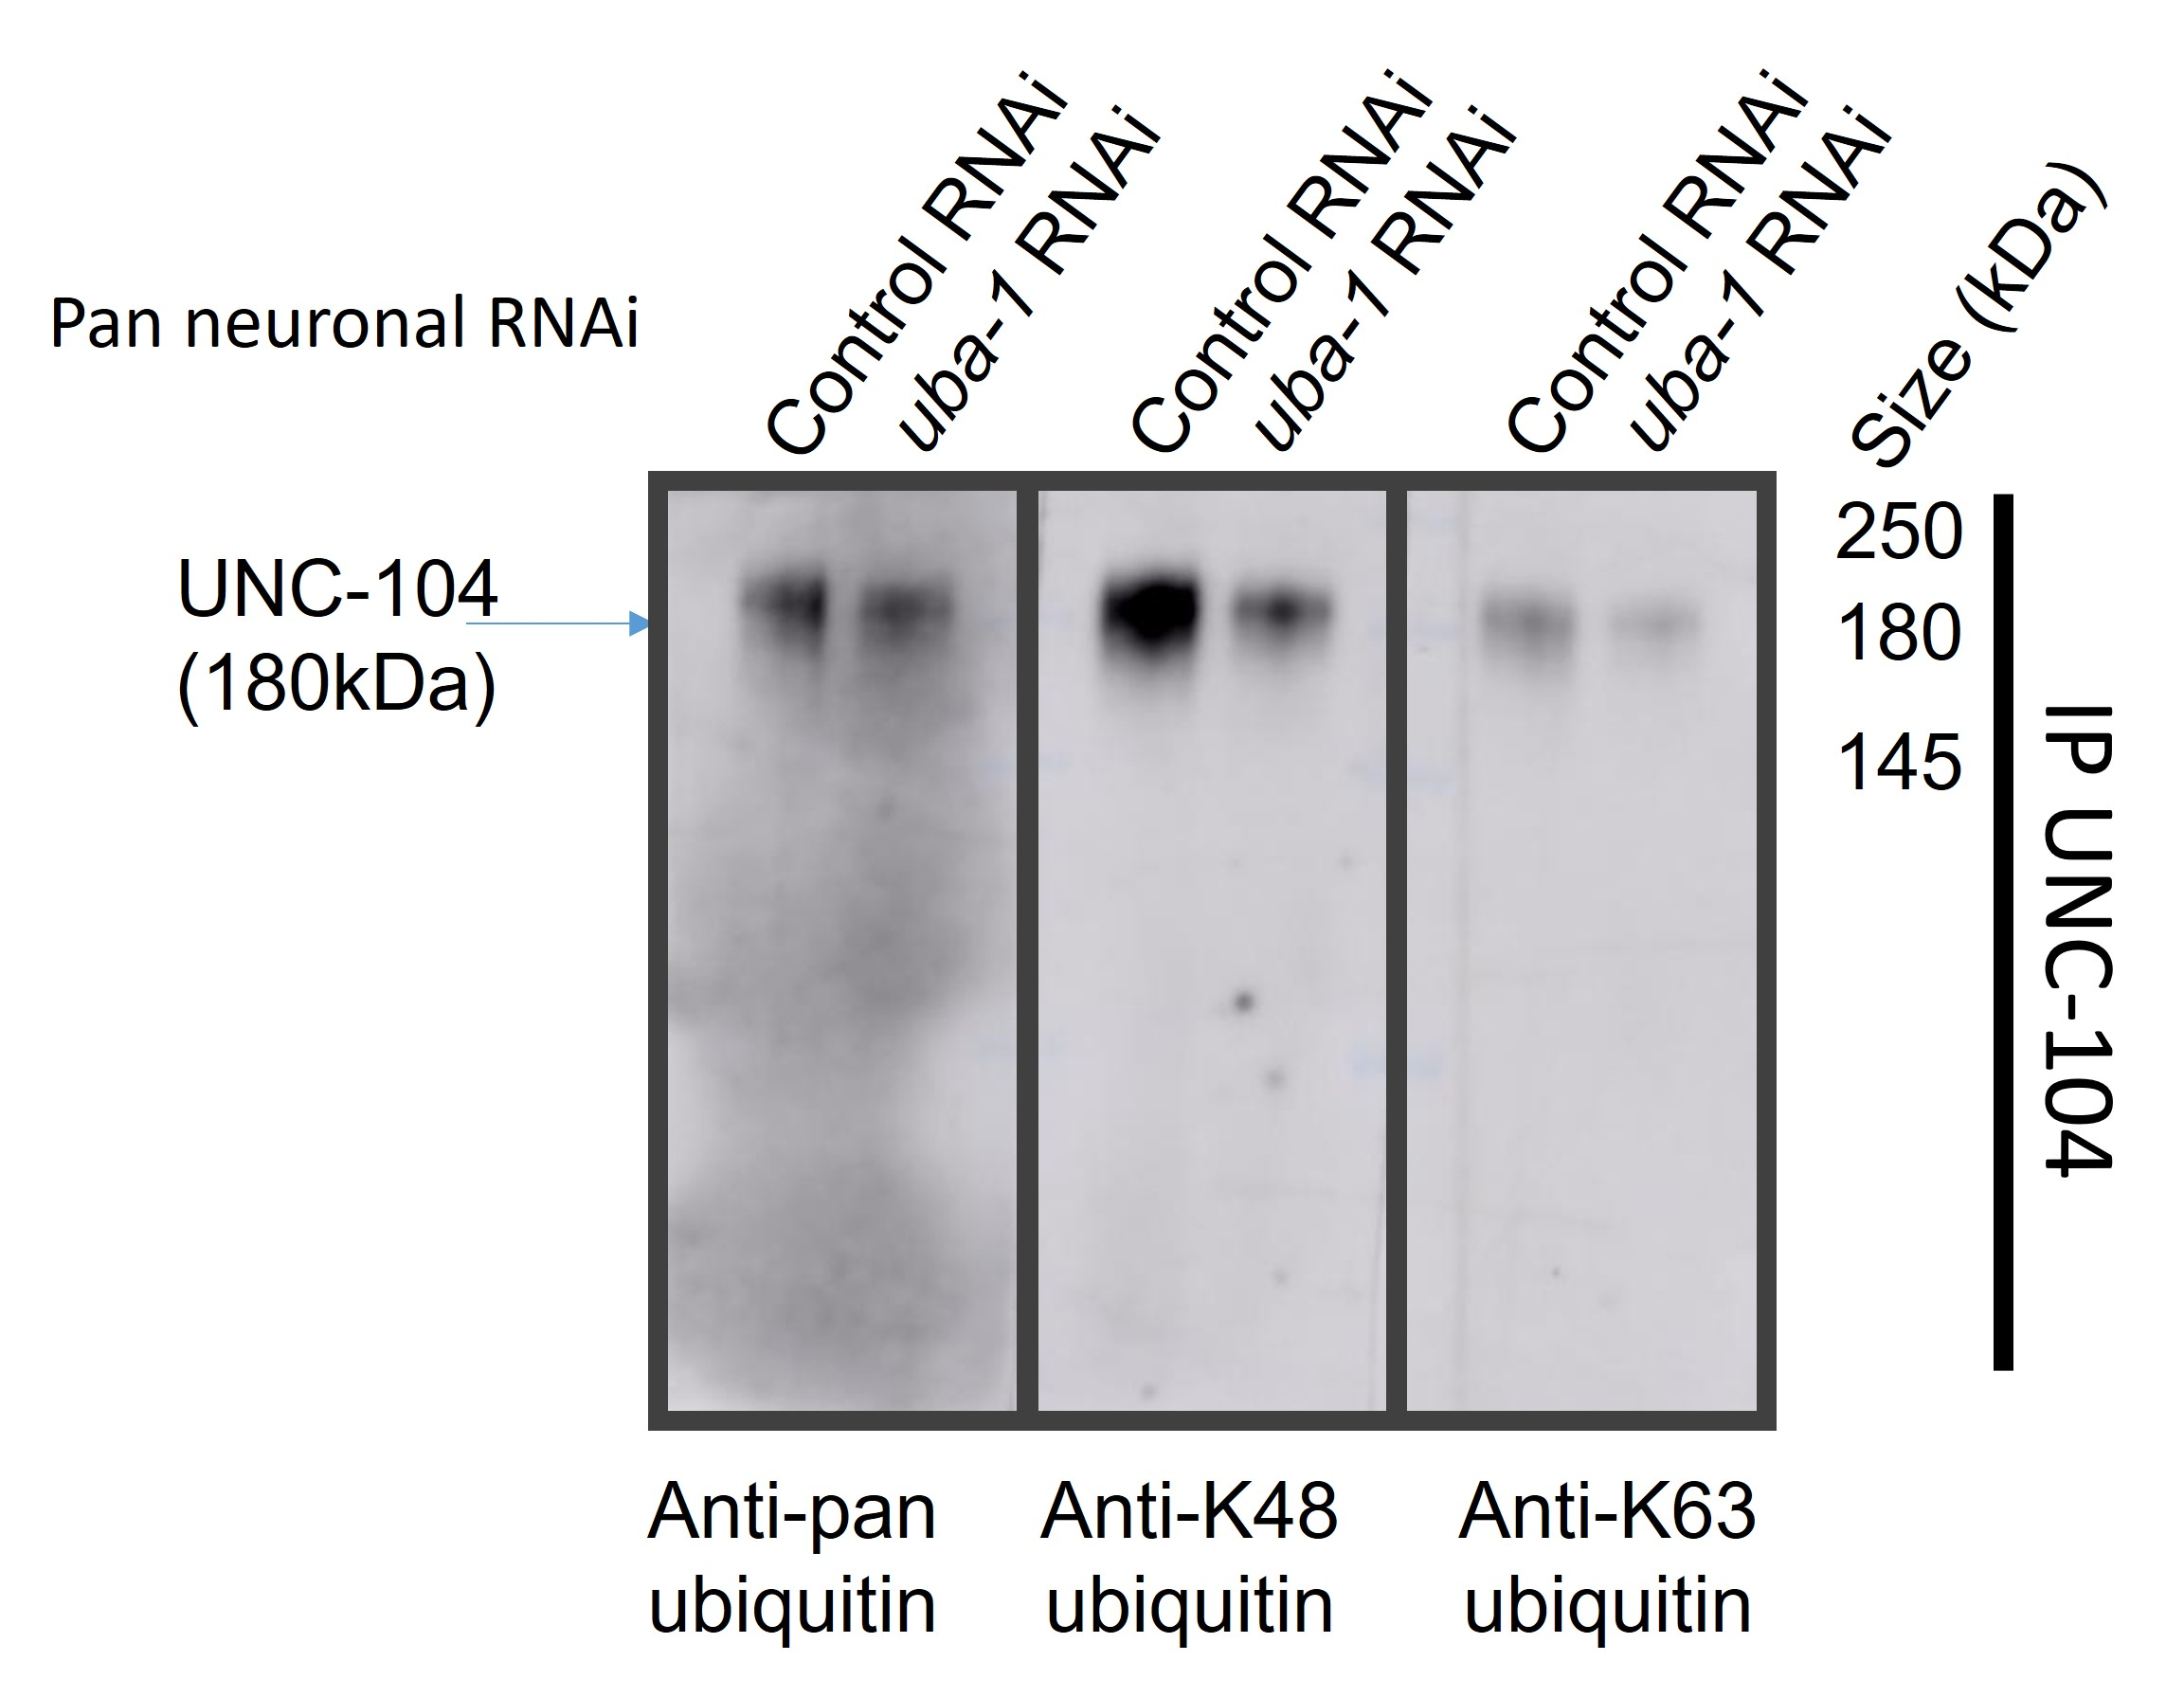
\includegraphics[width=1\linewidth]{figs/example}
	\caption[GFP::RAB-3 flux improves after successful fusion of the cut neuronal processes.]{\textbf{GFP::RAB-3 flux improves after successful fusion of the cut neuronal processes.}} \raggedright \small A) LASER based ablation of the PLM neuron expressing a soluble mCherry along with GFP::RAB-3, shows either a') growth of the proximal process followed by fusion, or b') growth of the proximal process with a failure in fusion with the distal process 24 hours post ablation. B) A schematic showing the traced neuronal processes from A). Representative kymographs of GFP::RAB-3 within the neuronal process with the cell body towards the right either proximal or distal to the cell body post-injury in a C) fusion successful, or D) fusion unsuccessful animal. Yellow arrow indicate anterograde particles, red arrow indicate retrograde particles and white arrow heads indicate stationary GFP::RAB-3 clusters. E) GFP::RAB-3 particle flux in the anterograde (A) or retrograde (R) directions within the proximal (Prox) or distal (Dist) neuronal process in animals with successful or unsuccessful fusion. F) GFP::RAB-3 particle flux in the anterograde (A) or retrograde (R) directions within the proximal (Prox) or distal (Dist) neuronal process in either wild type or \textit{let-7(lf)}. Bar graphs represent averages with the S.E.M. represented as whiskers. One-way ANOVA with Bonferroni test used for all statistical comparisons. ns- non significant, *p$<$0.05 ***p$<$0.001
	\label{fig:Atrayeerab}
\end{figure}

To observe if the fusion of the proximal and distal neuronal processes occurs just to establish cytoplasmic continuity, or if the cytoskeleton themselves are remodeled to create a seamless fusion point, we assessed GFP::RAB-3 movement across the fusion points [Fig.~\ref{fig:Atrayeemontage}]. We observed a smooth movement of GFP::RAB-3 across the fusion point suggesting that the increase in GFP::RAB-3 flux within the distal fragment arises from cargo transport from the proximal fragment.

\begin{figure}[H]
	\begin{minipage}[t]{0.45\textwidth}
%		\mbox{}\\[-\baselineskip]
		\vspace{0pt}
		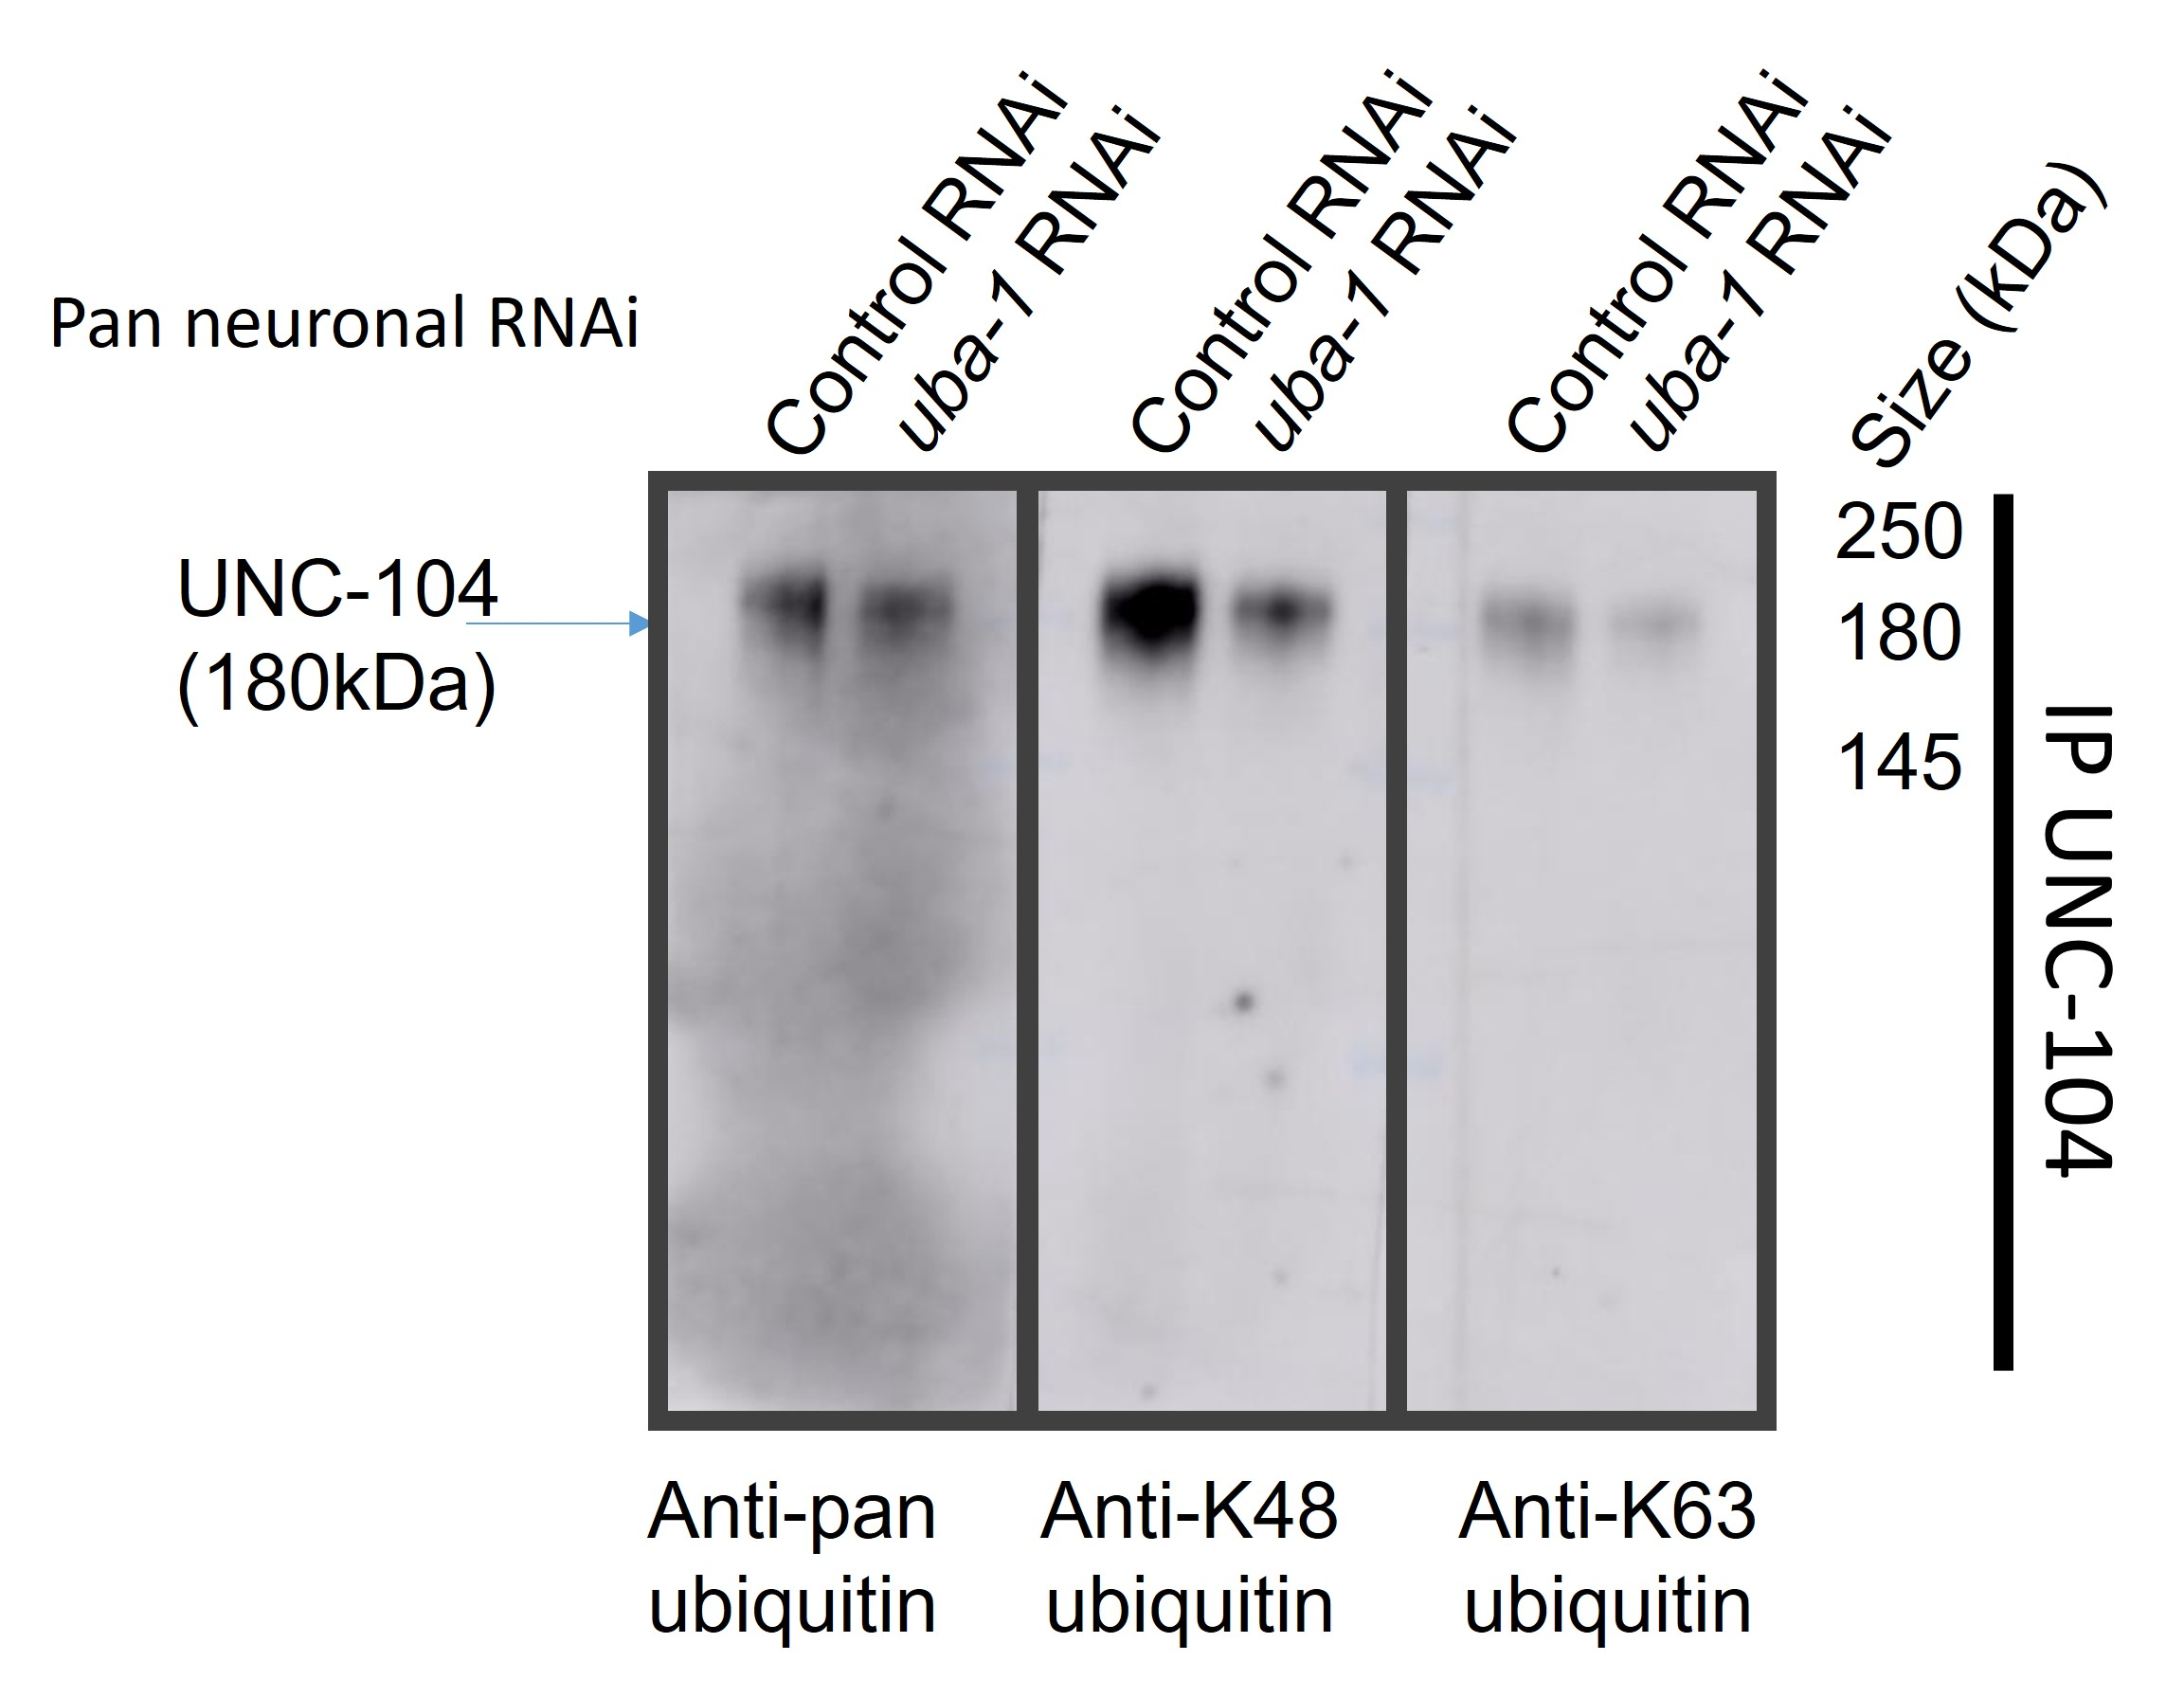
\includegraphics[width=\textwidth]{figs/example}
	\end{minipage}\hfill
	\begin{minipage}[t]{0.5\textwidth}
%		\mbox{}\\[-\baselineskip]
		\vspace{0pt}
		\caption[GFP::RAB-3 cargo movement across a successfully fused neuronal process post injury.]{\textbf{GFP::RAB-3 cargo movement across a successfully fused neuronal process post injury.}} \raggedright \small Montage showing portion of the PLM distal neuronal process expressing GFP::RAB-3 24 hour post injury, with the proximal process fusing in the middle of the distal process. The arrow head labels a single particle that seamlessly crosses the fusion point indicating cytoplasmic continuity between the proximal and distal ends of the neuronal process. Each frame is 250 ms apart. The proximal process, distal process and the fusion point are labeled with arrows. Cell body towards the right. \label{fig:Atrayeemontage}
	\end{minipage}
\end{figure}

	\newcolumntype{L}{>{\RaggedRight\hangafter=1\hangindent=1.5em}X}
	\begin{table}[H]\centering
		\caption{Strain list used in this study}\label{tab:StrainlistA}
		\scriptsize
		\begin{tabularx}{1\textwidth}{@{} l l L l @{}}\toprule
			S. No. &Strain name &Genotype &Reference \\\midrule
			1 &TT2464 &\textit{tbIs222} derived from UV integration of \textit{vdEx263}[(\textit{mec-4p}::\textit{mCherry} (5 ng/μl), \textit{odr-1p}::\textit{dsRed} (30 ng/μl)] &\cite{kirszenblat2013} \\
			2 &NM2689 &\textit{jsIs821} [\textit{mec-7p}::\textit{gfp}::\textit{rab-3}] &\cite{bounoutas2009} \\
			3 & &\textit{let-7(mg279)} &\cite{reinhart2000} \\
			\bottomrule
		\end{tabularx}
	\end{table}
	

\end{appendices}
 %Appendix section
	
\begin{appendices}
\chapter{Codes developed}




\begin{longlisting}
	\caption[Python code for generating initial list of all E3s]{Python code for generating initial list of all genes targeting E3 ligases. Requirements use Python2.7.
	\label{lst:E3list}}
	\inputminted{python}{codes/text_search2.py}
\end{longlisting}
\pagebreak
\begin{longlisting}
	\caption[Python code for getting FASTA files]{Python code for getting all FASTA files from wormbase using the gene names from the previous code as input. Requirements use Python2.7.
	\label{lst:E3fasta}}
	\inputminted{python}{codes/E3fasta.py}
\end{longlisting}


\pagebreak
\begin{longlisting}
	\caption[Jupyter notebook for visualizing RNAi screen data]{Jupyter notebook for visualizing RNAi screen data as a clustered heatmap. Requirements use Python3.8.
		\label{lst:RNAivisualize}}
	\fbox{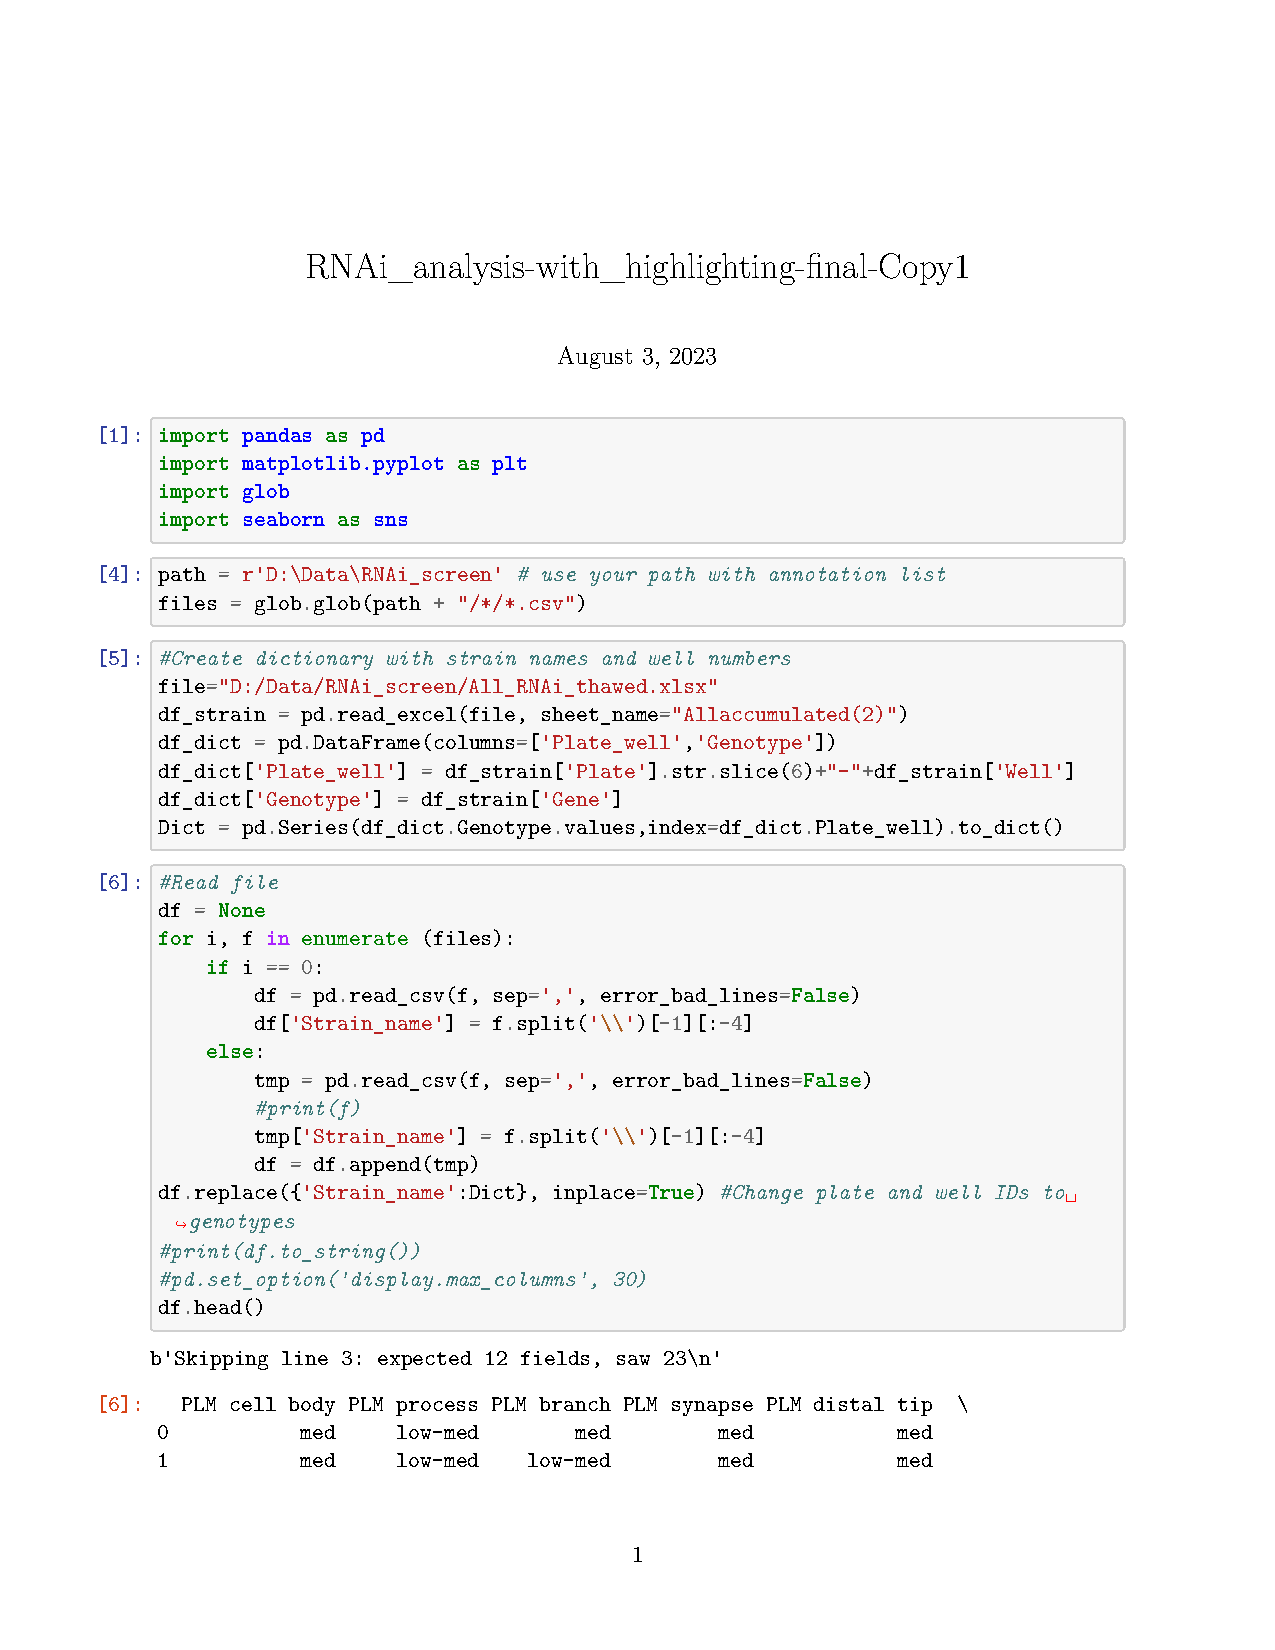
\includegraphics[page=1,scale=.78]{codes/RNAi_analysis-with_highlighting-final-Copy1.pdf}}
	\includepdf[pages=2-,frame=true,pagecommand={\pagestyle{headings}}, scale=0.8]{codes/RNAi_analysis-with_highlighting-final-Copy1.pdf}
\end{longlisting}

\end{appendices}
 %Codes
	

\begin{appendices}
\chapter{Directory information}



\begin{forest}
	pic dir tree,
	pic root,
	for tree={% folder icons by default; override using file for file icons
		directory,
	},
	[Data backup
		[Anusheela's Data for paper
			[qPCR data]
			[Final figures]
			[Analysis]
		]
		[Atrayee's data]
		[Dhruva's data]
		[DNA sequences
			[Sequencing]
			[Designing strategies]
			[Constructs available]
		]
		[Keertana's data]
		[Motor Degradation
			[Imaging]
			[Westerns]
			[Mol Bio]
			[qPCR]
			[RNAi list]
			[Codes]
			[Mass spec]
		]
		[Ritabhas's Data
			[fbxa-103]
			[branch imaging]
			[ATG9GFP]
			[AP3]
			[Analysis]
			[Illustrator files]
		]
		[Sucheta's data
			[Actin wyIs291]
			[Microtubule juIs338]
			[jsIs821]
		]
	]
\end{forest}





\begin{forest}
	pic dir tree,
	pic root,
	for tree={% folder icons by default; override using file for file icons
		directory,
	},
	[Motor Degradation
		[Imaging
			[Cargo Intensity
				[Static RAB-3 RNAi screen
					[Multiple folders for RNAi
						[Each folder contains files labeled w$\textunderscore$1 onwards, file]
					]
				]
				[Static RAB-3 with mutant and RNAi
					[sid-1-him-5-uIs71-tb120-jsIs821
						[EV]
						[1-F7]
						[2-F5]
						[Each folder contains files labeled w$\textunderscore$1 onwards, file]
					]
					[sid-1-him-5-uIs71-syd-2-jsIs821
						[EV]
						[1-F7]
						[2-F5]
						[Each folder contains files labeled w$\textunderscore$1 onwards, file]
					]
					[sid-1-him-5-uIs71-sam-4-jsIs821
					[EV]
					[1-A11]
					[1-F7]
					[2-F5]
					[uba-1]
					[UNC-104oe]
					[Each folder contains files labeled w$\textunderscore$1 onwards, file]
					]
				]
			]
		]
	]
\end{forest}

\end{appendices}
 %Directory information
	\bookmarksetup{startatroot} % Step 2: Add this line right before the references for correct hyperlinks
	\chapter*{References}
	\addcontentsline{toc}{chapter}{References}
	\printbibliography[heading=none]
\end{document}


